\documentclass{article}
\usepackage[utf8]{inputenc}
\usepackage{hyperref}
\usepackage{float}
\usepackage[table,xcdraw]{xcolor}
\usepackage{color, colortbl}
\usepackage{longtable}
%\usepackage[sort&compress,square,comma,authoryear]{natbib}
\usepackage{booktabs}
\usepackage{graphicx}
\usepackage{multirow}
\usepackage{tikz}
\usepackage{rotating}
% \graphicspath{{/home/kunz/Dokumente/Projects/Trait_DB/Invertebrate_traits/Paper/Figures/}}
\graphicspath{{Figures/}}
\usepackage{rotating}
\usepackage{geometry}
\usepackage{array}
\usepackage{lscape}
\usepackage{longtable}
\usepackage{hhline}
\usepackage{lmodern}
\usepackage[
backend = biber,
style = ieee,
citestyle = numeric-comp,
maxbibnames=99,
sorting = none % sort by name year title
]{biblatex}
\addbibresource{Ref_invertebrate_DB.bib}

\usepackage{subfiles} % Best loaded last in the preamble

% functions and definitions
\definecolor{Gray}{gray}{0.9}

% horizontal space between two columns
\setlength{\tabcolsep}{2mm}

\newcommand{\specialcell}[2][c]{%
  \begin{tabular}[#1]{@{}c@{}}#2\end{tabular}}

\renewcommand*{\thefootnote}{\alph{footnote}}


%%%%%%%%%%%%%%%%%%%%%%%%%%%%%%%%%%%%%%%%%%%%%%%%%%%%%%%%%%%%%%%%%%%%%%%%%%%%%%%%%%
%%%%%%%%%%%%%%%%%%%%%%%%%%%%%%%%%%%%%%%%%%%%%%%%%%%%%%%%%%%%%%%%%%%%%%%%%%%%%%%%%%
\title{DRAFT: Harmonized and trait aggregation paper }
\author{}%Stefan Kunz 
\date{}

\begin{document}
\maketitle

\section*{Introduction}

Explaining and predicting how communities are shaped by environmental factors is one of the main goals of ecology. Species traits, defined as measurable properties of an organism \cite{mcgill_rebuilding_2006}, might be beneficial in achieving this goal \cite{heino_jani_macroecological_2013}. Traits evolve through adaptations (e.g., physiological, behavioural, etc.) of organisms to their environment and indicate direct or indirect linkages between the biological response of an organism or a population and its environment \cite{southwood_habitat_1977, verberk_delivering_2013}.
Besides providing a mechanistic explanation of species-environment relationships, trait-based approaches might be suitable for large scale analysis because the variability in trait responses is lower than in taxonomic responses \cite{bonada_taxonomic_2007, baird_toward_2011}. Traits of freshwater invertebrate individuals are difficult to determine because - unlike plant traits - they often can not be measured directly. For example, to gain knowledge on feeding habits requires evaluating mouthpart morphology, consumed food, and the organisms function within its community \cite{moog_comprehensive_nodate}. Nevertheless, invertebrate traits have been increasingly used in freshwater ecology, e.g. by relating macroinvertebrate trait composition to environmental factors and as trait metrics in biomonitoring \cite{poff_developing_2010, szocs_effects_2014, bhowmik_large_2015, menezes_beyond_2010}.

In the last decades, freshwater ecologists have compiled comprehensive invertebrate trait databases for various continents \cite{usseglio-polatera_biomonitoring_2000, schmidt-kloiber_www.freshwaterecology.info_2015, vieira_database_nodate, Philips_and_Smith_NZ_DB_2018, kefford_integrated_2020, tomanova_trophic_2006}. The availability of invertebrate trait data from different continents enables comparisons of trait variation and analyses of their relation to environmental factors across large scales. However, such analyses have been carried out mostly within continents, using information from one or two trait databases. For example, Bonada et al. \cite{bonada_taxonomic_2007} compared trait composition for Mediterranean and temperate regions in Europe using traits from Usseglio-Polatera et al. \cite{usseglio-polatera_biomonitoring_2000}(typically referred to as Tachet database); Poff et al. \cite{poff_developing_2010} characterized trait composition across sites in the Western US using traits from Poff et al. \cite{poff_functional_2006}, and Botwe et al. \cite{botwe_effects_2018} investigated the effect of salinity on invertebrate traits in different sites in South Australia using trait data from Poff et al. \cite{poff_functional_2006} and Schäfer et al. \cite{schafer_trait_2011}. Analyses of invertebrate traits that synthesize information on invertebrate grouping features from more than two different continents are rare. 

In this study, we follow the terminology proposed by Schmera et al., where a grouping feature is defined as a general property (e.g. feeding mode) that comprises a "group of related traits (e.g., predator, shredder, etc.) that vary among species or among individuals within a species" \cite{schmera_proposed_2015}. Thus, we use the term grouping feature in place of which many studies use the term "trait", and the term trait instead of "trait state", "modality" or "trait category". Traits can be described using different codings (binary, fuzzy) that represent the prevalence of a characteristic in an organism.
% TODO: bring affinity/affinity scores in
% Could say that we call the proportionate description (0-1) "affinity" 

To our knowledge, only Brown et al. \cite{brown_functional_2018} harmonized grouping features from more than two geographically distant invertebrate trait databases, for a limited set of grouping features (8) and taxa (112), in a study on the influence of decreasing glacier cover on functional diversity and community assembly of invertebrates. 

We suspect that the heterogeneity of information in freshwater invertebrate trait databases, besides the diversity of taxa across regions, is likely a major reason for the lack of studies across continents. To harmonize grouping features from different regions, first commonly accepted and unambiguous trait definitions are required \cite{schneider_towards_2019}. In the best case, grouping features would be classified into the same traits across databases or they could easily be harmonized using standardized terminology. However, a lack of standardized terminology of trait definitions and poor metadata quality in many trait databases are common issues throughout the field of trait-based ecology \cite{baird_toward_2011, schneider_towards_2019}. Secondly, consistent coding of traits facilitates the compatibility of trait data from different databases. 

% Alternative from Ben:
Traits can be described in a binary fashion, or with multiple categories, ignoring uncertainty how the trait is expressed in any particular organism (e.g. adult terrestrial stage, presence of gills) or continuous (e.g. tolerance of pollution, body size). One approach for dealing with uncertainty is the use of fuzzy coded variables, where the traits are assigned probabilistic values. Fuzzy codes are used to account for plasticity in traits, variability in traits within taxonomic groups above species, and incomplete knowledge and are usually converted to proportions. % TODO: add affinitiy scores here?

However, invertebrate trait databases are heterogeneous regarding the coding they use for their traits \cite{culp_incorporating_2011}. Brown et al. \cite{brown_functional_2018} harmonized grouping features based on trait databases from Europe, North America, and New Zealand because in these trait databases identical grouping features are classified differently into traits. As the traits from North America were coded binary in contrast to the traits from Europe and New Zealand which have been established using affinity scores, the authors consulted experts to assign fuzzy coded traits to North American taxa or inferred them from the European trait database. Thus, it becomes apparent that using invertebrate trait data from several regions requires extensive data processing prior to the actual data analysis. A centralized database with standardized and unambiguous traits and a consistent coding of traits would minimize data processing effort.
Discrepancies in the taxonomic resolutions (e.g. species, genus or family) when linking observational taxonomic data to trait database represents another challenge. When observations are on a more precise taxonomic level than data available in the trait databases (e.g. observations on species-level, trait data on genus-level) trait information of the less precise taxonomic level is often assigned (e.g. \cite{szocs_effects_2014, vos_taxonomic_2017}). Conversely, if trait information is only available on more precise taxonomic levels than the observed taxa, traits are aggregated to a less precise taxonomic level, e.g. \cite{poff_functional_2006, szocs_effects_2014, piliere_a._f._h._importance_2016, aspin_extreme_2019}. Studies have used different methods of trait aggregation, e.g. the mean \cite{magliozzi_functional_2019}, median \cite{szocs_effects_2014} or the mode \cite{piliere_a._f._h._importance_2016}. Up to now, studies on how and to which extent different trait aggregation methods influence trait-based analysis are missing. However, related knowledge would inform future studies regarding the choice of the aggregation method.

% TODO: clarify, see Ralf's comment
The necessity to aggregate and harmonize trait data due to the discrepancies in trait definitions motivated us to compare different trait aggregation methods and evaluate whether the harmonization of trait data ...
As a basis for our analysis, we (1) established 4 novel invertebrate trait datasets consisting of  7 grouping features based on trait databases from Europe, North America, Australia, and New Zealand. To evaluate different trait aggregation methods we (2) compared trait affinities obtained through different trait aggregation methods to trait affinities assigned at family-level by experts for two of the established trait datasets. % Mention simulation
(3) To evaluate how harmonizing grouping features and aggregating traits can modify results of trait-environment relationships we re-analysed data on the effect of anthropogenic salinisation on biological traits by Szöcs et al. \cite{szocs_effects_2014} using trait data from the established harmonized European trait datasets. By comparison with the original analysis, we investigated how harmonizing and aggregating trait data can modify the outcome of trait-environment relationships. Finally, we (4) present an overview of discrepancies in trait definition between the used invertebrate trait datasets and discuss challenges of trait data synthesis.


\newpage
%%%%%%%%%%%%%%%%%%%%%%%%%%%%%%%%%%%%%%%%%%%%%%%%%%%%%%%%%%%%%%%%%%%%%%%%%%%%%%%%%%%%%%%%%%%%%%%%%%%%%

\section*{Methods}

\subsection*{Selection of traits and harmonization of trait databases}

We extracted information from 6 trait databases from Europe, North America, Australia, and New Zealand and harmonized 7 grouping features. Trait information for Europe was obtained from the freshwaterecology.info database \cite{schmidt-kloiber_www.freshwaterecology.info_2015} and the Tachet database \cite{usseglio-polatera_biomonitoring_2000}. The freshwaterecology.info contains taxa on species-level, while taxa recorded in the Tachet database are on species, genus and family-level. Trait information for North America was obtained from Twardochleb et al. \cite{twardochleb_trait_data_2020} and complemented by Vieira et al. \cite{vieira_database_nodate}. Data on body form for European and North American taxa was based on expert knowledge \cite{polatera_personal_information_2020}. For Australia and New Zealand, we used trait databases from Kefford et al. \cite{kefford_integrated_2020} and Philips and Smith respectively \cite{Philips_and_Smith_NZ_DB_2018}. To increase readability we refer to the databases as well as the datasets we extracted from them by the name of the continent they originate from, except for European databases, which we refer to by their commonly used names (freshwaterecology.info and Tachet database). 
 
We selected traits of seven grouping features that were available in all databases, are commonly applied in trait-based ecological studies, and describe different parts of the biology of a species: life history (Voltinism), morphology (Respiration, Body form, Size), ecology (Locomotion, Feeding mode) and reproduction (Oviposition). We omitted ecological traits that describe habitat preferences (e.g. temperature preference) because these traits are missing in the New Zealand trait database. The grouping features were differently classified across the databases, we therefore harmonized them into 26 traits (Table \ref{tab:traits_harmonization}). Harmonization was undertaken by amalgamating similar traits into one trait (e.g. crawlers and sprawlers into crawlers). Thereby, for a particular taxa the highest trait affinity score among the amalgamated traits was taken. 

We used fuzzy coded traits for establishing our harmonized datasets unless data quality prohibited. In the latter case we used binary traits, i.e. categorical and continuous traits were converted into binary traits. For example, in the  freshwaterecology.info database, the classification of the trait voltinism accounts for different faunistic regions. Hence, entries such as "arctic" or "boreal" of e.g. the trait univoltine were substituted with a value of 1. Implicitly, we assumed for binary traits that a value of 1 and 0 corresponds to the highest and no affinity for a particular trait. Fuzzy codes are reported with different ranges in the trait databases (e.g. freshwaterecology.info 0 to 10, Tachet database 0 to 3 or 0 to 5). We standardized these to a range between 0 and 1 and converted trait affinities to percentages. Thus, fuzzy coded and binary traits were in the same range. 

Prior to harmonization we consolidated duplicate taxa on species, genus or family-level if present within a dataset, by either applying the median for fuzzy coded traits, or the maximum for binary traits. We omitted taxa with a lower taxonomic precision than family-level.

\begin{table}[H]
\centering
\caption{Traits of the harmonized grouping features. The last column indicates traits that were amalgamated for harmonization (no amalgamation needed if empty).}
\label{tab:traits_harmonization}
\begin{tabular}{lll}
\toprule[.1em]
Grouping feature & Trait & Amalgamated traits\\
\toprule[.1em]
Voltinism    & \begin{tabular}[c]{@{}l@{}}Semivoltine\\ Univoltine\\ Bi/multivoltine\end{tabular}                                & \begin{tabular}[c]{@{}l@{}}\textless 1 generation per year\\ 1 generation per year\\ \textgreater 1 generation per year\end{tabular}                                                                                                                                            \\
\midrule
Body Form    & \begin{tabular}[c]{@{}l@{}}Cylindrical \\ Flattenend\\ Spherical\\ Streamlined\end{tabular}                       & \begin{tabular}[c]{@{}l@{}}Cylindrical, tubular\\ Flattenend, dorsoventrally flattened \textsuperscript{\textit{a}}\\ Spherical, round (humped)\\ Streamlined, fusiform\end{tabular}                                                                                                                                                                          \\
\midrule
Size         & \begin{tabular}[c]{@{}l@{}}Small \\ Medium \\ Large\end{tabular}                                                  & \begin{tabular}[c]{@{}l@{}}\textless 9 mm, \textless 10 mm \textsuperscript{\textit{b}}\\ 9 - 16 mm, 10 - 20 mm\\ \textgreater 16 mm, \textgreater 20 mm\end{tabular}                                                                                                                \\
\midrule
Respiration  & \begin{tabular}[c]{@{}l@{}}Gills\\ Plastron/Spiracle\\ \\ \\ \\ Tegument\end{tabular}                             & \begin{tabular}[c]{@{}l@{}} Tracheal gills, gills\\ Temporary air store, Spiracular gills, \\ atmospheric breathers, plant breathers, \\ functional spiracles, air (plants), aerial, \\ plastron/spiracle\\ Cutaneous, tegument \end{tabular}                                                                         \\
\midrule
Locomotion   & \begin{tabular}[c]{@{}l@{}}Burrower\\ Crawler\\ Sessile\\ Swimmer \end{tabular}                                     & \begin{tabular}[c]{@{}l@{}}Interstitial, boring, burrowing\\ Sprawler, walking, climber, clinger, crawler\\ Attached, sessile\\ Skating, diving, planctonic, swimming\end{tabular}                                                                                                                 \\
\midrule
Feeding mode & \begin{tabular}[c]{@{}l@{}}Filterer\\ \\ Gatherer\\ \\ Herbivore\\ \\ Parasite\\ Predator\\ Shredder \\ \\ \end{tabular} & \begin{tabular}[c]{@{}l@{}}Active/passive filterer, absorber, \\ filter-feeder, collector-filterer, filterer\\ Deposit-feeder, collector-gatherer, \\ detrivore, gatherer\\ Grazer, scraper, piercer herbivore, \\ herbivore, algal piercer, piercer (plants)\textsuperscript{\textit{c}}\\ \\ Piercer (animals)\textsuperscript{\textit{c}}, predator \\ Miner, xylophagus, shredder, \\ shredder detrivore\end{tabular} \\
\hline
Oviposition  & \begin{tabular}[c]{@{}l@{}}Aquatic eggs\\ \\ Ovoviviparity\\ Terrestrial eggs\end{tabular}                            & \begin{tabular}[c]{@{}l@{}}Eggs attached to substrate/plants/stones,\\ free/fixed eggs/clutches\\ \\ Terrestrial clutches, terrestrial \end{tabular}     \\
\bottomrule[.1em]
\end{tabular}
\end{table}
\begin{minipage}{\linewidth}{\fontsize{8}{10}\selectfont
    \textit{a} The trait "bluff (blocky)" occurred in the Vieira et al. \cite{vieira_database_nodate} database and was newly classified by expert knowledge into cylindrical and flattened \cite{polatera_personal_information_2020}. \\  
    \textit{b} Reflects the different size classifications by the North American trait databases and the other trait databases. \\
    \textit{c} The trait piercer was defined in the Tachet database for piercing plants and animals, in contrast to the other databases \cite{usseglio-polatera_biomonitoring_2000}. Taxa exhibiting this trait have been assigned to predators or herbivores based on expert knowledge \cite{polatera_personal_information_piercer_2020}.
}
\end{minipage}

\newpage
%%%%%%%%%%%%%%%%%%%%%%%%%%%%%%%%%%%%%%%%%%%%%%%%%%%%%%%%%%%%%%%%%%%%%%%%%%%%%%%%%%%%%%%%%%%%%%%%%%%%%

\subsection*{Trait aggregation}

Traits of the harmonized grouping feature datasets were aggregated to family-level using three approaches. I) Direct aggregation of taxa to family-level giving equal weight to every taxon using the mean or median, denoted \textit{direct\_agg\textsubscript{mean}} and \textit{direct\_agg\textsubscript{median}}, respectively. II) Stepwise aggregation, i.e. first to the genus-level and subsequently to the family-level using the mean or median. This approach gives equal weights to each genus. Hereafter, we denote this aggregation type as \textit{stepwise\_agg\textsubscript{mean}} or \textit{stepwise\_agg\textsubscript{median}}, respectively. III) Aggregation using a weighted mean approach, denoted as \textit{weighted\_agg}. This method weights the genera according to the number of their species in the trait datasets regardless if for every used grouping feature information was available (Figure \ref{fig:data_proc_overview}). 

To examine the influence of the taxonomic hierarchy and the trait variability on the outcome of the different trait aggregation methods we created three hypothetical examples of different taxonomic hierarchies. 
1) A family with an equal number of genera and species (5 genera each with 5 species respectively), denoted as \textit{sim\_base}.
2) A family where one genus has a much larger number of species than the other 4 genera (1 genus with 13 species, 4 genera with 3 species respectively), denoted as \textit{sim\_extreme}. 
3) A family where all genera have a different number of species (8, 2, 7, 3, 5), denoted as \textit{sim\_variation}. In total every family consisted of 25 species. To each hypothetical taxonomic hierarchy a hypothetical grouping feature with 3 traits was assigned. The 25 affinities for each trait were simulated by sampling from a truncated normal distribution with a mean value of 0.5 and 5 levels of standard deviations (0.2, 0.4, 0.6, 0.8, and 1) respectively to simulate different levels of trait variability. The truncated normal distribution was bound to 0 and 1. Simulated trait affinities were converted to percentages, similar to the data processing of the trait databases. The sampling was repeated 100 times for each standard deviation. Hence, in total 100 datasets for each level of trait variability were simulated, resulting in 12500 simulated trait affinities ($25$ species per family $* 5$ levels of trait variability $* 100$ replicates). All trait aggregation methods were applied to each simulated dataset. The results were compared based on the produced range of aggregated trait affinities between levels of trait variability and hypothetical taxonomic hierarchies. We also compared for each simulated dataset the differences in trait affinities obtained by each aggregation method.  

\begin{figure}
  \centering
  \subfile{Flowchart/Flowchart_methods.tex}
  \caption{Data processing steps of the selected traits. Intermediate (gray) and main (orange) steps of data preparation are depicted. The dashed bottom box illustrates the different trait aggregation methods using a small made-up example (data in the upper left corner). The aggregation methods (blue) and intermediate steps of the aggregation methods (purple) are displayed. Abbreviations: EU: Europe, NOA: North America, AUS: Australia, NZ: New Zealand, DB: Database.}
  \label{fig:data_proc_overview}
\end{figure}

%%%%%%%%%%%%%%%%%%%%%%%%%%%%%%%%%%%%%%%%%%%%%%%%%%%%%%%%%%%%%%%%%%%%%%%%%%%%%%%%%%%%%%%%%%%%%%%%%%%

\subsection*{Comparison of family-level aggregated traits with family-level assigned traits}

Aggregated trait affinities of the five trait aggregation methods (\textit{direct\_agg\textsubscript{median}}, \textit{direct\_agg\textsubscript{mean}}, \textit{stepwise\_agg\textsubscript{median}}, \textit{stepwise\_agg\textsubscript{mean}}, and \textit{weighted\_agg}) were compared to trait affinities assigned at family-level by experts, which were available for Australia and North America for a subset of grouping features and taxa. For the Australian dataset, we compared aggregated trait affinities with assigned trait affinities resolved at family-level for the grouping features feeding mode and size using data from Chessman et al. \cite{chessman_dissolved-oxygen_2018}. In Chessman et al. \cite{chessman_dissolved-oxygen_2018} feeding mode is classified similarly as in the Australian dataset except that the trait parasite is missing. We conducted the comparison for the 220 families available in Chessman et al. \cite{chessman_dissolved-oxygen_2018}. Considering each factor combination of family and trait (in total 8) this amounts to 1760 cases.

For the North American dataset, we compared aggregated trait affinities with assigned trait affinities on family-level for the grouping features feeding mode, respiration, size, voltinism, and locomotion. The assigned trait affinities at family-level are part of the North American database (Twardochleb et al.) \cite{twardochleb_trait_data_2020} and originate from expert knowledge. Trait information was available for 94 families of which all were present in the North American dataset (total number of cases 1598). The traits were on the categorical scale and were converted to binary traits prior to the comparison with aggregated trait affinities.

As mentioned above, trait affinities ranged from 0 to 1. Hence, the maximum difference possible in trait affinities is 1 or -1 (corresponds to 100 \%). For convenience and to improve interpretation, we report absolute trait differences.

%%%%%%%%%%%%%%%%%%%%%%%%%%%%%%%%%%%%%%%%%%%%%%%%%%%%%%%%%%%%%%%%%%%%%%%%%%%%%%%%%%%%%%%%%%%%%%%%%%%%%

\subsection*{Analysis of the effect of harmonization and trait aggregation on trait-environment relationships}

We repeated the analysis of Szöcs et al. \cite{szocs_effects_2014} who studied the effect of anthropogenic salinization on invertebrates in the River Werra in Germany. For the re-analysis we used the established harmonized grouping features for Europe and additionally aggregated traits using the aforementioned aggregation methods. 

The river Werra has been subject to effluents from the potash industry since the mid of the 20th century and allows to study responses of invertebrates and their trait compositions to salinization \cite{bathe_biological_2011}. Sites downstream, upstream, and close to the salt discharge (transition) were compared regarding their trait composition. Further details can be found in Szöcs et al. \cite{szocs_effects_2014}. 

We substituted 6 of the grouping features from the original data with harmonized grouping features from the European trait dataset. We compared the results of the redundancy analysis (RDA) from the original study to the case when using harmonized grouping features. Specifically, the trait composition expressed as community weighted mean (CWM) traits was ordinated along an electric conductivity gradient. We compared the species scores obtained from the RDA, i.e. the coordinates of the tips of the vectors representing the CWM traits in the bi- or triplots. Following the original study, we identified traits associated with high or low salinity based on their distance to the ordination axis median using the mahalanobis distance. Traits with a mahalanobis distance greater than the $97.5 \%$ -quantile of the Chi-square distribution (5.02) were regarded as traits responding to either low or high salinity. For our analysis, we used the same 21 grouping features that Szöcs et al. \cite{szocs_effects_2014} used. The 6 harmonized grouping features used were \textit{Size, Feeding mode, Locomotion, Oviposition, Respiration}, and \textit{Voltinism}. Additionally, for testing the effect of aggregated traits we assigned to each taxon in Szöcs et al. \cite{szocs_effects_2014} the aggregated trait value for its corresponding family and repeated the RDA.  

%%%%%%%%%%%%%%%%%%%%%%%%%%%%%%%%%%%%%%%%%%%%%%%%%%%%%%%%%%%%%%%%%%%%%%%%%%%%%%%%%%%%%%%%%%%%%%%%%%%%%

\subsection*{Data analysis}

The data processing and aforementioned analyses were carried out using R (Version 3.6.1). Raw data and the R code for data processing and grouping feature harmonization is located in the Github repository: \url{https://github.com/KunzstLD/Invertebrate_traits}. Scripts and data to reproduce the trait aggregation and analysis with aggregated traits are located in the Github repository \url{https://github.com/KunzstLD/Trait-aggregation}.

%%%%%%%%%%%%%%%%%%%%%%%%%%%%%%%%%%%%%%%%%%%%%%%%%%%%%%%%%%%%%%%%%%%%%%%%%%%%%%%%%%%%%%%%%%%%%%%%%%%%

\newpage
\section*{Results}

\subsection*{Taxonomic coverage of the harmonized trait datasets}

Regarding the taxonomic coverage, the New Zealand dataset has the smallest taxon pool (478 taxa, Table \ref{tab:tax_coverage}). By contrast, the European trait dataset has the largest taxon pool with 4601 taxa followed by the North American trait dataset that contained trait information on 3753 taxa. The Australian dataset contains 1402 taxa. The European, New Zealand, and North American datasets have most taxa on the species-level whereas the Australian dataset has a similar number of taxa on species and genus-level.

\begin{table}[ht]
    \centering
    \caption{Number of taxa per harmonized dataset and per taxonomic level. Numbers in parenthesis show rounded relative frequencies in percentage.} 
    \label{tab:tax_coverage}
    \begin{tabular}{lccccc}
    \toprule[.1em]
    Database & Nr. of taxa & Species & Genus & Family & Nr. aquatic insects \\ 
    \toprule[.1em]
    EU & 4601 & 3739 (81) & 704 (15) & 158 (3) & 3942 (86) \\ 
    NOA & 3753 & 2414 (64) & 1163 (31) & 176 (5) & 3305 (88) \\ 
    AUS & 1402 & 564 (40) & 578 (41) & 260 (19) & 1016 (72) \\ 
    NZ & 478 & 404 (85) & 47 (10) & 27 (6) & 443 (93) \\ 
    \bottomrule
    \end{tabular}
\end{table}

%%%%%%%%%%%%%%%%%%%%%%%%%%%%%%%%%%%%%%%%%%%%%%%%%%%%%%%%%%%%%%%%%%%%%%%%%%%%%%%%%%%%%%%%%%%%%%%%%%%%

\subsection*{Completeness of trait information}

The amount of entries with available information for the selected grouping features varied strongly for the preprocessed European, North American, and Australian datasets (Table \ref{tab:trait_coverage}). By contrast, the New Zealand dataset contained complete trait information for most of the investigated grouping features (between 94 \% and 100 \%).

\begin{table}[ht]
    \centering
    \caption{Rounded percentage of entries that have 
    information for the individual grouping features
    shown per trait dataset.} 
    \label{tab:trait_coverage}
    \begin{tabular}{lccccccc}
    \toprule[.1em]
    Database & Body form & Oviposition & Voltinism & Locomotion & Size & Respiration & Feeding mode \\ 
    \toprule[.1em]
    EU & 8 & 15 & 23 & 36 & 11 & 57 & 76 \\ 
    NOA & 28 & 13 & 47 & 52 & 73 & 44 & 63 \\ 
    AUS & 4 & 46 & 49 & 39 & 75 & 68 & 99 \\ 
    NZ & 100 & 94 & 100 & 99 & 100 & 100 & 99 \\ 
    \bottomrule
    \end{tabular}
\end{table}

\newpage

%%%%%%%%%%%%%%%%%%%%%%%%%%%%%%%%%%%%%%%%%%%%%%%%%%%%%%%%%%%%%%%%%%%%%%%%%%%%%%%%%%%%%%%%%%%%%%%%%%%%

\subsection*{Simulation of varying taxonomic hierarchies}

We evaluate the simulation results based on the produced range of aggregated trait affinities and by comparing results of every simulated dataset. 

The trait aggregation methods \textit{direct\_agg\textsubscript{mean}}, \textit{direct\_agg\textsubscript{median}} and \textit{weighted\_agg} yielded similar ranges of aggregated trait affinities within each level of trait variability for the \textit{sim\_base} scenario. The \textit(stepwise\_agg \textsubscript{median}) and \textit(direct\_agg \textsubscript{median}) yielded mostly greater ranges of aggregated trait affinities for the \textit{sim\_base} scenario. As expected with increasing trait variability the produced range of trait affinities increased (Figure \ref{fig:overview_sim_results}). By contrast, the ranges of trait affinities slightly differed for all aggregation methods for the simulation scenarios \textit{sim\_extreme} and \textit{sim\_variation}. \textit{Weighted\_agg} and \textit{stepwise\_agg\textsubscript{mean}} produced a wider range of trait affinities than the \textit{direct\_agg\textsubscript{mean}} in the \textit{sim\_extreme} scenario. For most levels of trait variability the \textit{stepwise\_agg \textsubscript{median}} resulted in the largest range of trait affinities in the \textit{sim\_extreme} and \textit{sim\_variation} scenarios.

% 10 unique comparisons, 100 datasets, 5 levels of trait variability, 3 sim scenarios  
A comparison of the results of the aggregation methods for each simulated data set showed that in most simulated datasets the differences between the aggregated traits were small. Only 1.42 \% (213 out of 15.000) of all comparisons showed a difference equal or greater than an absolute trait affinity of 0.1. Most of these differences occurred for the \textit{sim\_extreme} scenario (83.5 \%). The majority of the differences equal or above 0.1 were found between the aggregation methods \textit{direct\_agg\textsubscript{mean}} and \textit{stepwise\_agg\textsubscript{median}}, \textit{direct\_agg\textsubscript{median}} and \textit{stepwise\_agg\textsubscript{median}}, and \textit{stepwise\_agg\textsubscript{median}} and \textit{weighted\_agg} (Figure S\ref{fig:sim_indv_runs}). 
% Differences were rather small, largest difference 0.265 for sim_extreme (stepwise_median vs weighted_agg) 

Overall, differences between the results of the aggregation methods for each simulated dataset increased with increasing trait variability. According to the simulation results, the different aggregation methods often result in similar trait affinities.  If differences occurred, than mostly between aggregation methods using the median and aggregation methods using the mean. 


\begin{figure}[H]
  \centering
  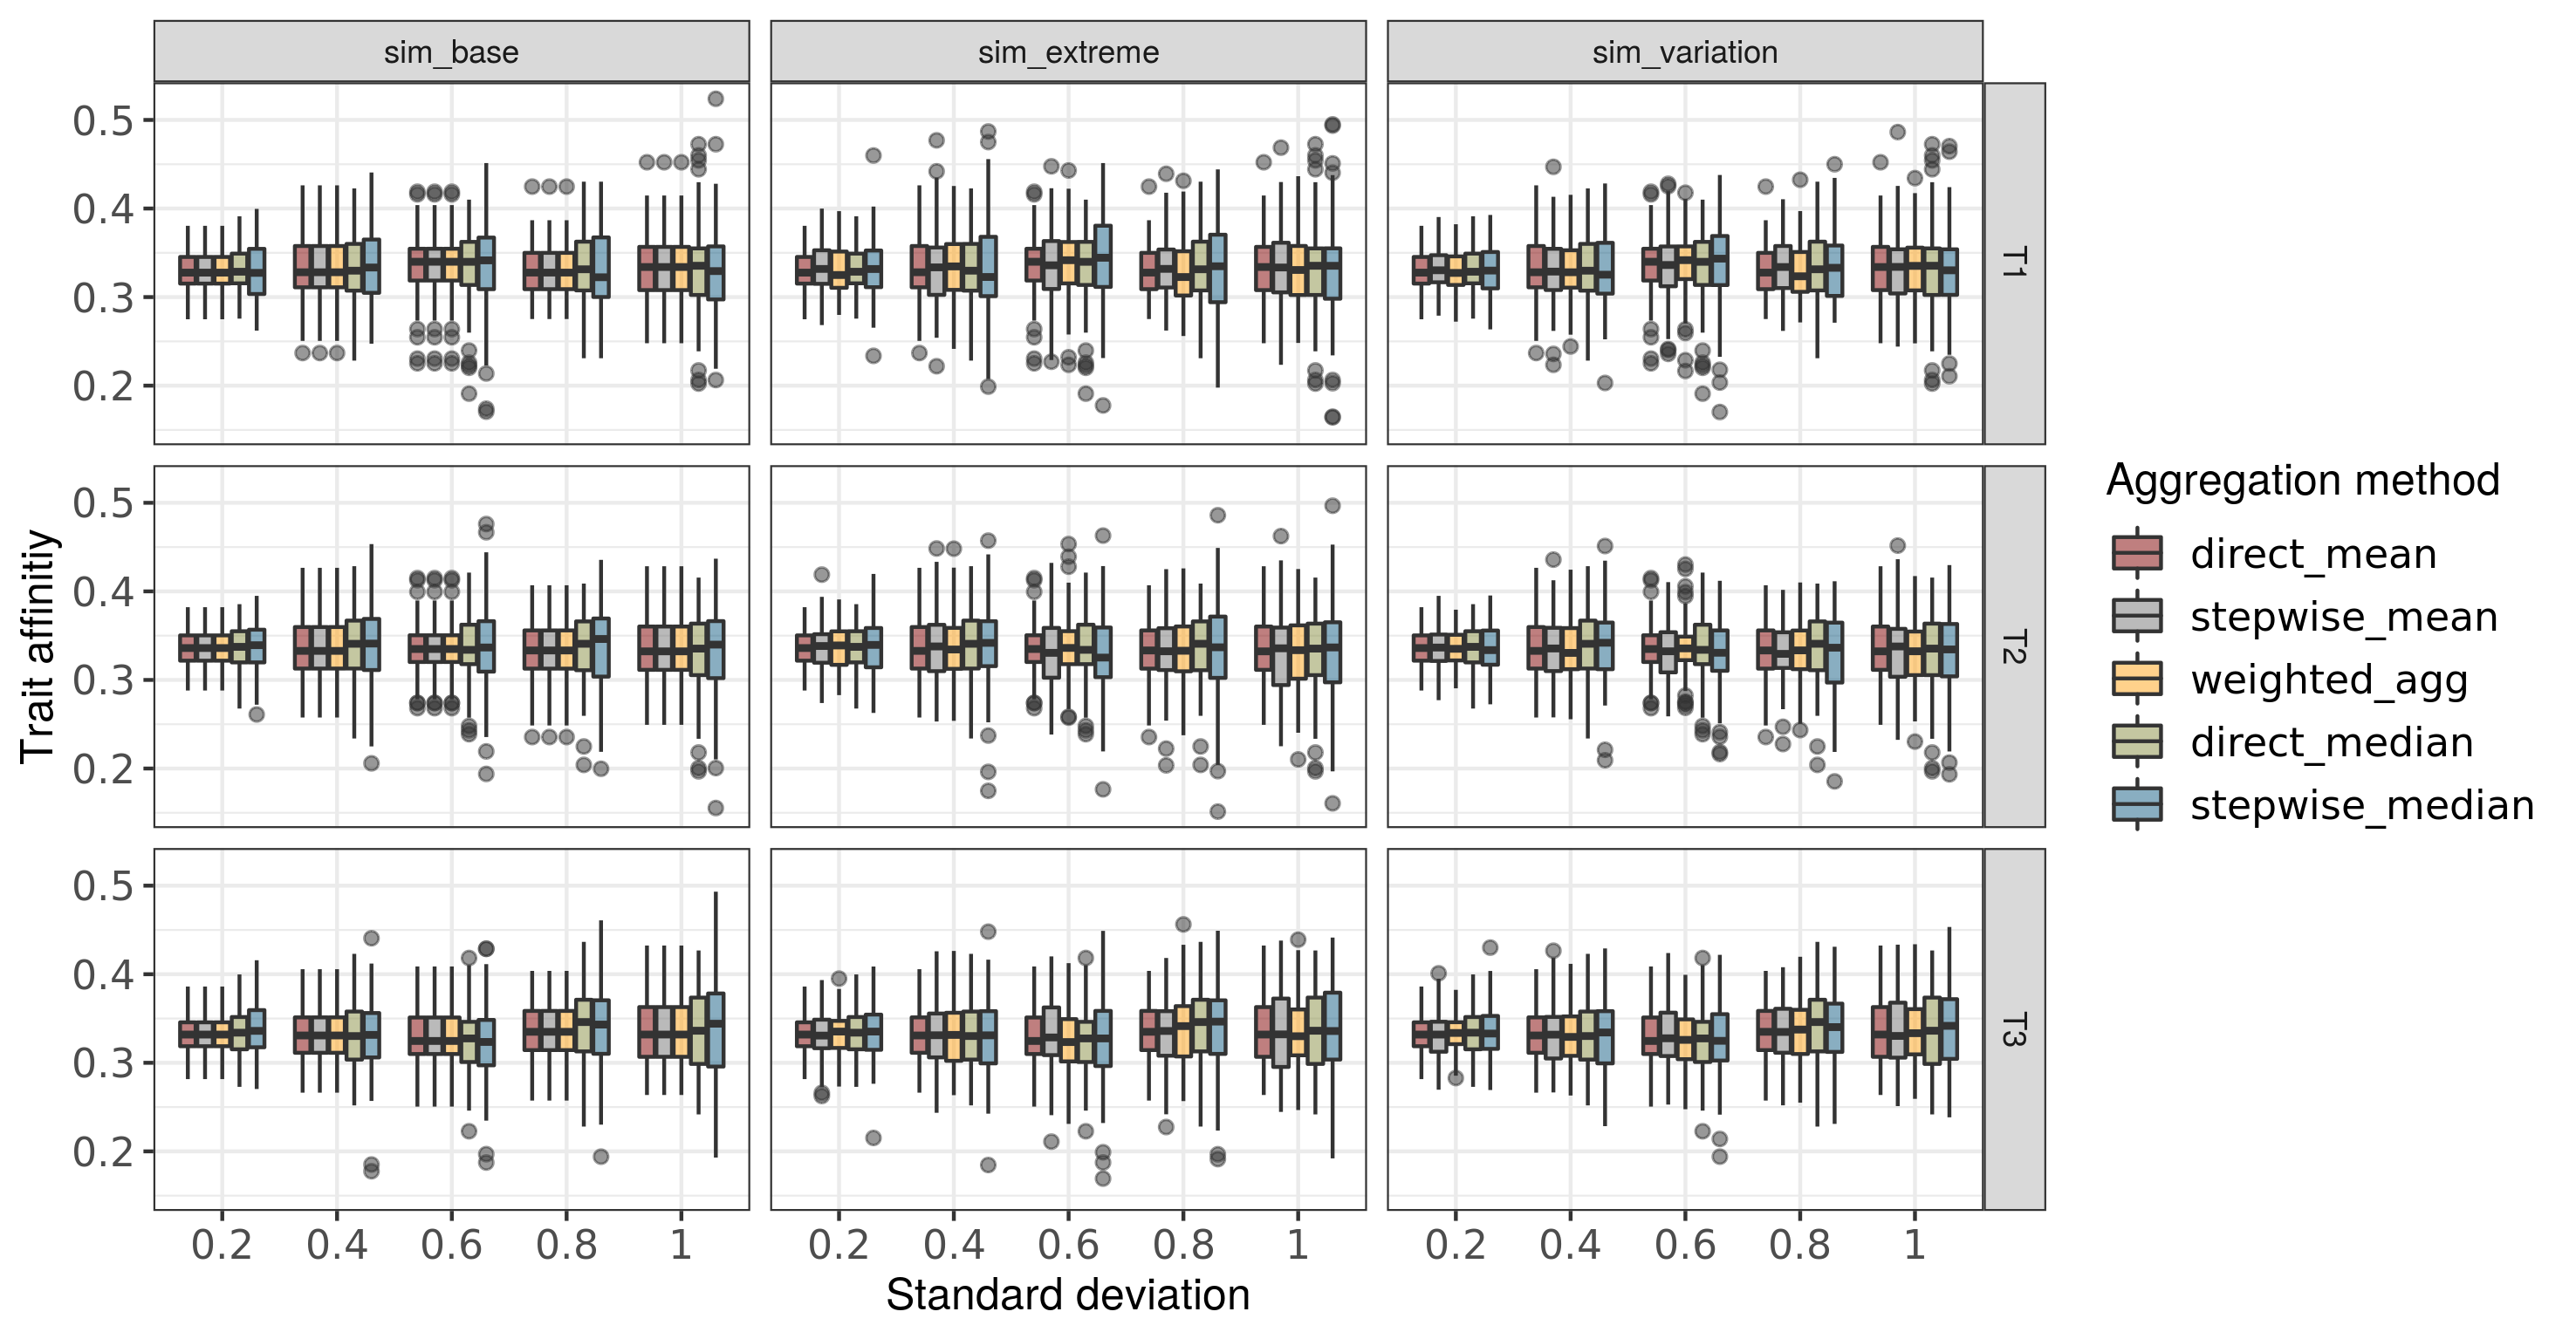
\includegraphics[width=16.5cm, height=10cm]{Overview_sim_results.png}
  \caption{Ranges of aggregated trait affinities for the three examples of taxonomic hierarchies and simulated levels of trait variability. Boxplots depict results for each trait aggregation method of 100 simulations. T1, T2, and T3 are the simulated traits.}
  \label{fig:overview_sim_results}
\end{figure}

\begin{figure}[H]
  \centering
  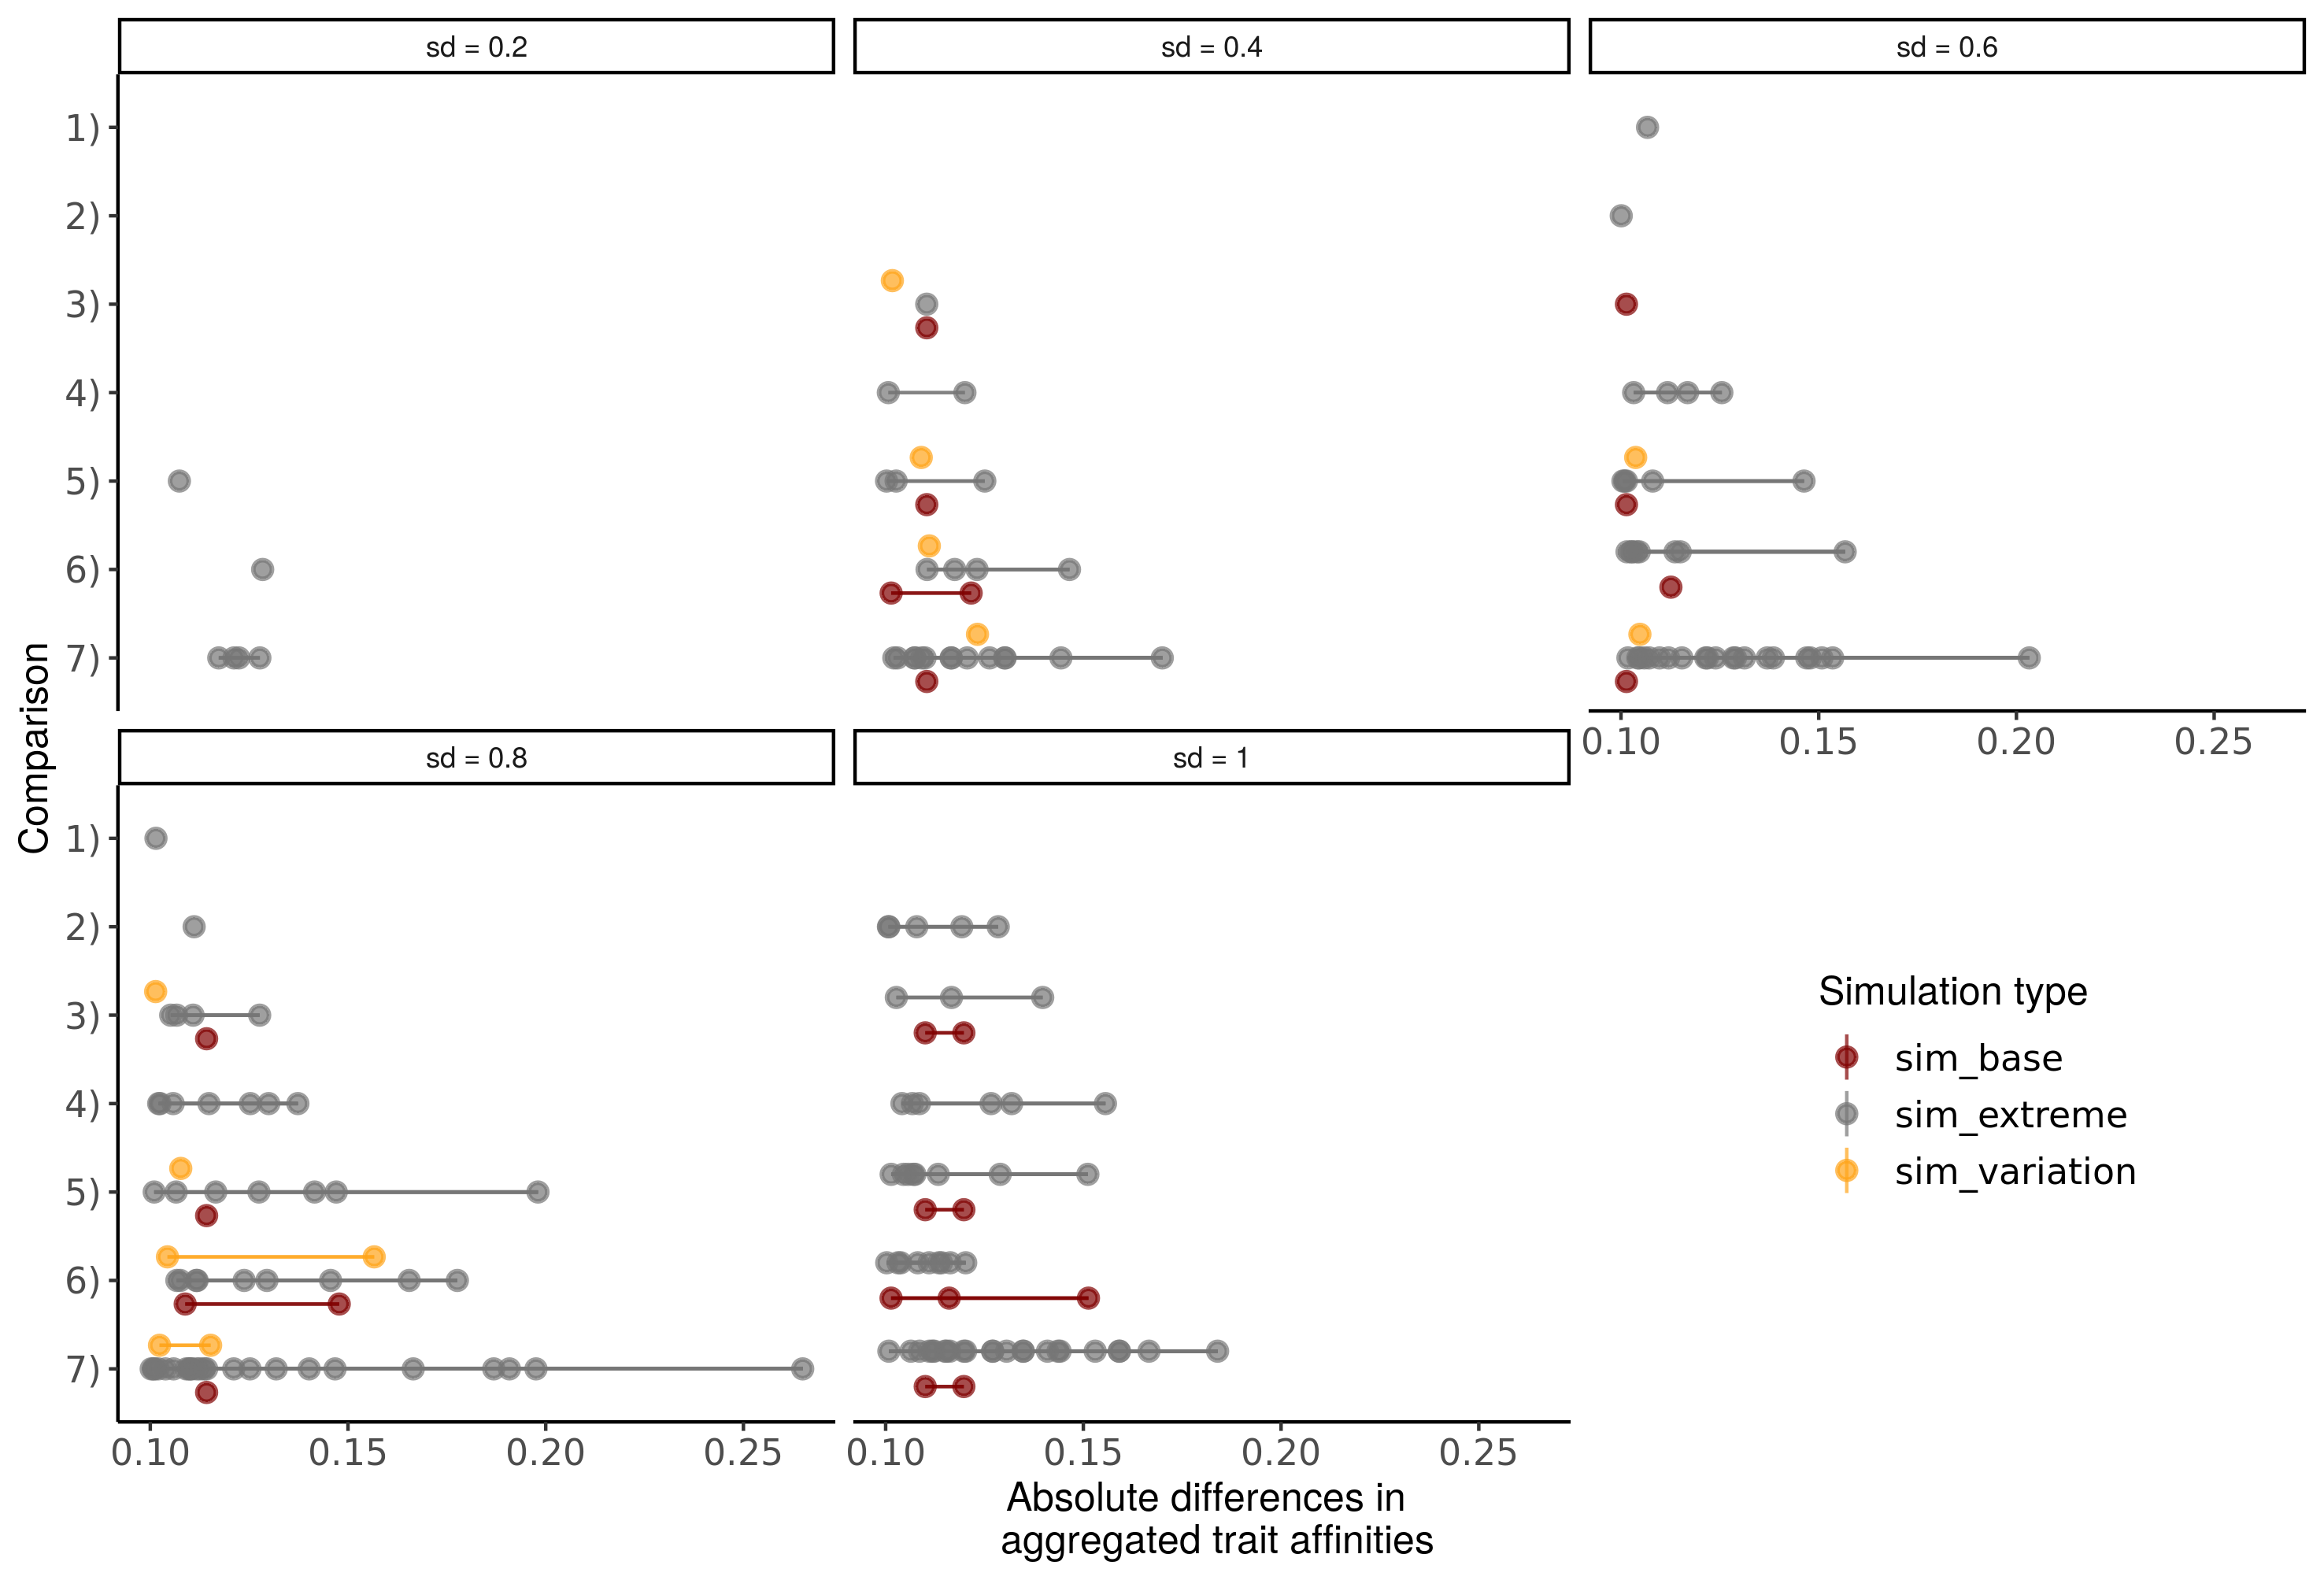
\includegraphics[width=16.5cm, height=10cm]{Diffs_indiv_runs_sim.png}
  \caption{Comparison of the aggregated trait affinities produced by the different trait aggregation methods for every simulated dataset across all 3 simulated traits. Dots depict comparisons where absolute differences between aggregated trait affinities were greater than 0.1. \newline
  Comparison: \newline
  1) Direct\_agg (median) - Stepwise\_agg (mean) \newline
  2) Direct\_agg (median) - Weighted\_agg, \newline
  3) Stepwise\_agg (mean) - Stepwise\_agg (median), \newline
  4) Stepwise\_agg (mean) - Weighted\_agg, \newline  
  5) Direct\_agg (mean) - Stepwise\_agg (median), \newline
  6) Direct\_agg (median) - Stepwise\_agg (median), \newline
  7) Stepwise\_agg (median) - Weighted\_agg \newline
  }
  \label{fig:sim_indv_runs}
\end{figure}

\newpage

\subsection*{Differences in trait affinities obtained by trait aggregation methods compared to traits assigned at family-level}
\label{sec:diff_trait_agg_chessman}

The percentage of differing cases of trait affinities obtained by the trait aggregation methods compared to trait affinities originally assigned at family-level varied between 16.2 \% and 22.9 \% for the Australian dataset. For the North American dataset, comparison of the trait aggregation methods to trait affinities assigned at family-level yielded between 15.3 \% and 47 \% differing cases (Table \ref{tab:summary_stat_aggr_vs_fam_assigned}). In general, trait aggregation methods using the median yielded fewer cases with differences compared to approaches using the mean. However, aggregation methods using the median produced greater differences for both datasets. Standard deviations of absolute differences were similar for all tested aggregation methods. For both datasets maximum differences of 1 occurred for all investigated grouping features (Figure \ref{fig:diff_aggr_traits_chessman} and Figure \ref{fig:diff_aggr_traits_pyne}).

% Is that necessary?
A comparison of the aggregation methods with each other for the 4 datasets revealed that differences in aggregated trait affinities were largest between the \textit{stepwise\_agg\textsubscript{median}} and \textit{direct\_agg\textsubscript{median}} (Figure S\ref{fig:comp_aggr_methods}).

\begin{table}[H]
  \centering
  \caption{Amount of differing cases, the minimum and maximum, and means and standard deviations of absolute differences between trait affinities assigned at family-level and aggregated trait affinities.}
  \label{tab:summary_stat_aggr_vs_fam_assigned}
  \begin{tabular}{ll|ccccc}
  \toprule[.1em]
  Database & \specialcell{Comparison to\\ traits at fam.-lvl.} & \specialcell{Differing \\ cases [\%]} & \specialcell{Min. \\ differences} & \specialcell{Max. \\ differences} & \specialcell{Mean abs. \\ differences} & \specialcell{SD abs. \\ differences} \\ 
  \toprule[.1em]
  \multirow{4}{*}{\specialcell{Australia \\ (Chessman)}} & \specialcell{direct\_agg (median)} & 16.53 & 0.01 & 1.00 & 0.45 & 0.27 \\ 
  & \specialcell{direct\_agg (mean)} & 23.24 & $< 0.01$ & 0.99 & 0.34 & 0.23 \\ 
  & \specialcell{stepwise\_agg (median)} & 17.90 & 0.01 & 1.00 & 0.42 & 0.26 \\ 
  & \specialcell{stepwise\_agg (mean)} & 23.24 & $< 0.01$ & 0.99 & 0.33 & 0.22 \\ 
  & \specialcell{weighted\_agg} & 23.24 & $< 0.01$ & 1.00 & 0.34 & 0.24 \\ 
  \midrule
  \multirow{4}{*}{\specialcell{North America}} & \specialcell{direct\_agg (median)} & 15.33 & 0.17 & 1.00 & 0.70 & 0.26 \\ 
  & \specialcell{direct\_agg (mean)} & 47.00 & $< 0.01$ & 1.00 & 0.30 & 0.26 \\ 
  & \specialcell{stepwise\_agg (median)} & 18.00 & 0.08 & 1.00 & 0.63 & 0.28 \\ 
  & \specialcell{stepwise\_agg (mean)} & 47.00 & $< 0.01$ & 1.00 & 0.30 & 0.27 \\ 
  & \specialcell{weighted\_agg} & 47.00 & $< 0.01$ & 1.00 & 0.31 & 0.28 \\ 
  \bottomrule
  \end{tabular}
\end{table}

\newpage

\begin{figure}[H]
  \centering
  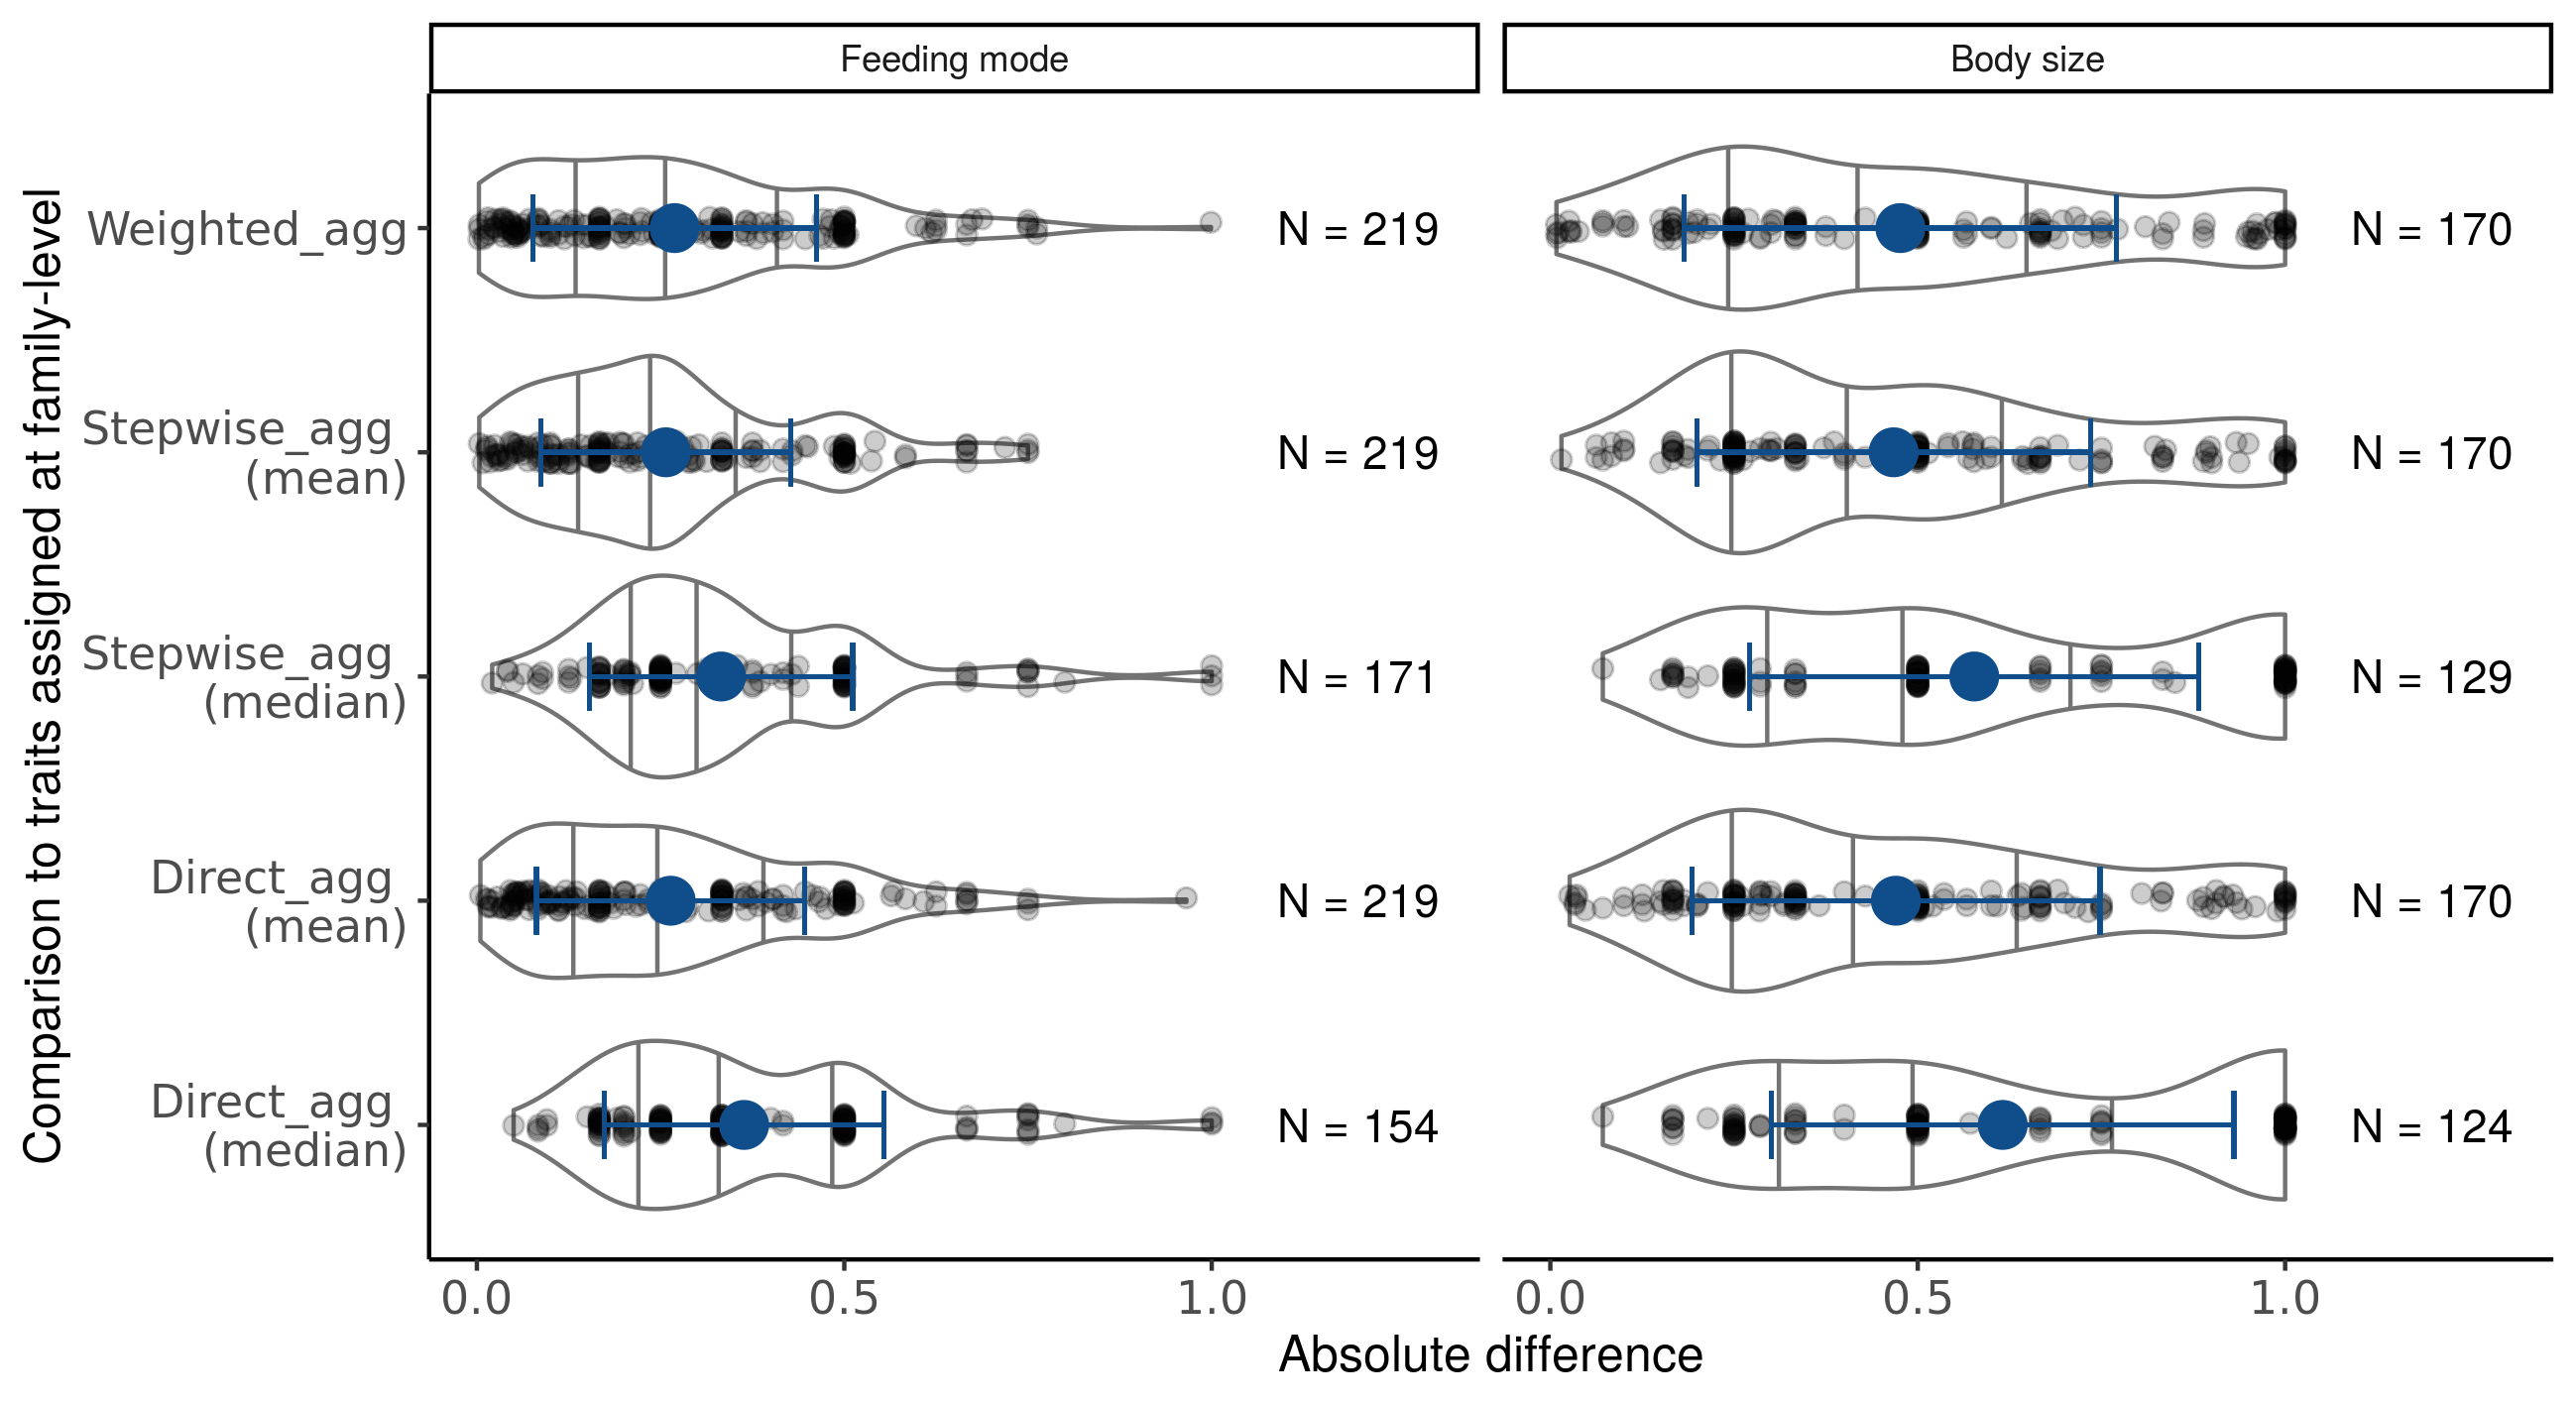
\includegraphics[width=16.5cm, height=10cm]{Deviances_trait_agg_chessman.png}
  \caption{Display of the cases (factor combination investigated families and traits) where differences occurred between aggregated traits and traits assigned at family-level. Violin plots - a mirrored density plot - show the density of the absolute trait affinity differences for the Australian dataset for the grouping features feeding mode and body size. Absolute differences in trait affinities are depicted as gray dots. N denotes the number of cases per comparison where differences occurred. The blue dot indicates the mean of absolute differences and the error bars the standard deviation. The gray vertical lines show the 25th, 50th and 75th quantile of the density estimate.}
  \label{fig:diff_aggr_traits_chessman}
\end{figure}


\begin{figure}[H]
  \centering
  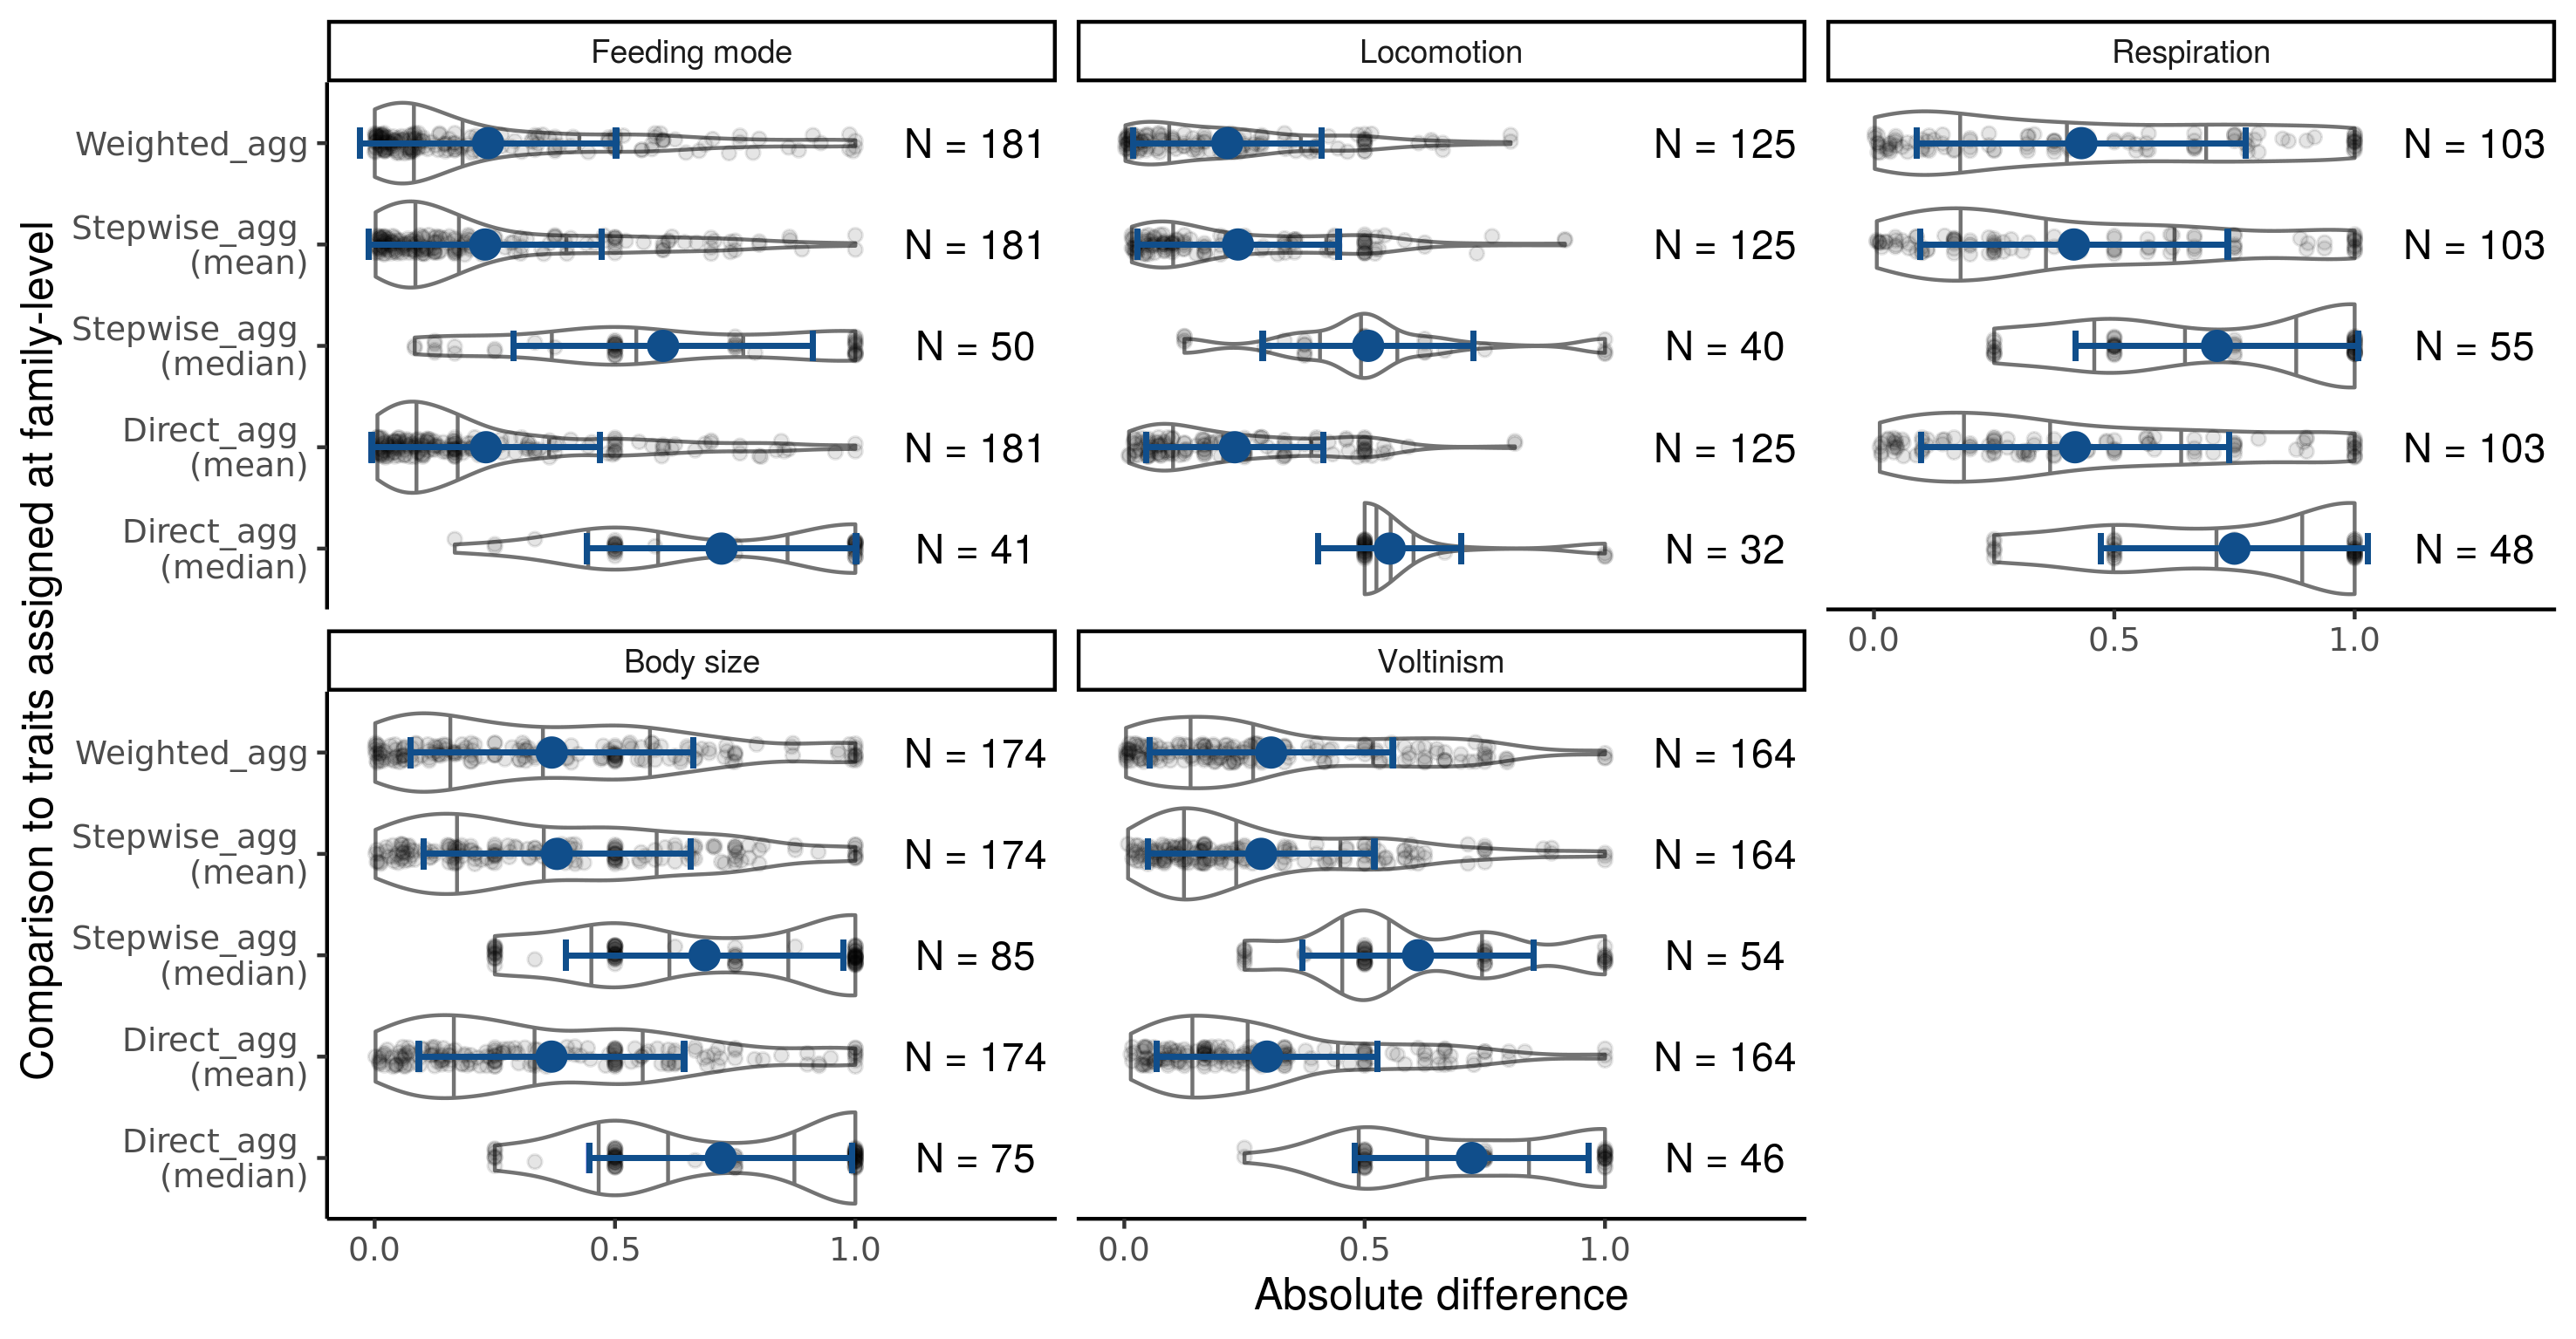
\includegraphics[width=16.5cm, height=10cm]{Deviances_trait_agg_pyne.png}
  \caption{Display of the cases (factor combination investigated families and traits) where differences occurred between aggregated traits and traits assigned at family-level. Violin plots - a mirrored density plot - show the density of the absolute trait affinity differences for the North America dataset for the grouping features feeding mode, locomotion, respiration, body size and voltinism. Absolute differences in trait affinities are depicted as gray dots. N denotes the number of cases per comparison where differences occurred. The blue dot indicates the mean of absolute differences and the error bars the standard deviation. The gray vertical lines show the 25th, 50th and 75th quantile of the density estimate.}
  \label{fig:diff_aggr_traits_pyne}
\end{figure}

\newpage 

%%%%%%%%%%%%%%%%%%%%%%%%%%%%%%%%%%%%%%%%%%%%%%%%%%%%%%%%%%%%%%%%%%%%%%%%%%%%%%%%%%%%%%%%%%%%%%%%%%%%

\subsection*{Re-analysis of Szöcs et al. using harmonized and aggregated grouping features}

The original RDA in Szöcs et al. \cite{szocs_effects_2014} indicated that downstream sites (high salinity) were characterised by the traits shredder, ovoviviparity, multivoltinism, long life cycle ($> 1$ year), and gill respiration and upstream sites (low salinity) were characterized by univoltinism, oviposition in clutches and short life cycle duration ($< 1$ year). 

Using harmonized grouping features resulted in fewer traits that distinguish upstream and downstream sites in comparison to the original analysis (Figure \ref{fig:rda_species_scores} and Figure \ref{fig:boxplots_scores_on_constrained_axis}). According to the RDA of the trait composition, downstream sites were characterised by taxa with the traits multivoltinism and ovoviviparity and upstream sites were characterised by univoltine taxa that lay their eggs in an aquatic environment (aquatic eggs). The traits shredder, gill respiration and long life cycle duration did not characterise sites with high salinisation. Also, the trait short life cycle duration did not characterise upstream sites with low salinity.

Using at family-level aggregated traits from the harmonized dataset showed results similar to the original analysis (Figure \ref{fig:rda_species_scores} and Figure \ref{fig:boxplots_scores_on_constrained_axis}). The \textit{direct\_agg\textsubscript{mean}}, \textit{direct\_agg\textsubscript{median}}, and \textit{weighted\_agg} 
characterised the downstream sites with the same traits as the original analysis except that downstream sites were not characterised by the trait shredder. Upstream sites were characterised by the traits univoltinism, aquatic eggs and short life cycle duration. The trait aquatic eggs of the harmonized grouping feature oviposition has been derived by amalgamating the trait oviposition in clutches and other related traits (Table \ref{tab:traits_harmonization}). The same results were obtained when re-analysing the data with traits aggregated by the \textit{stepwise\_agg\textsubscript{mean}} and \textit{stepwise\_agg\textsubscript{median}}, with the exception that none of the life cycle traits characterised upstream or downstream sites. Thus, in our comparison the direct and weighted family-level aggregation methods yielded to the least change in species scores of all methods compared to the original results.

\begin{figure}[H]
    \label{fig:rda_species_scores}
    \centering
    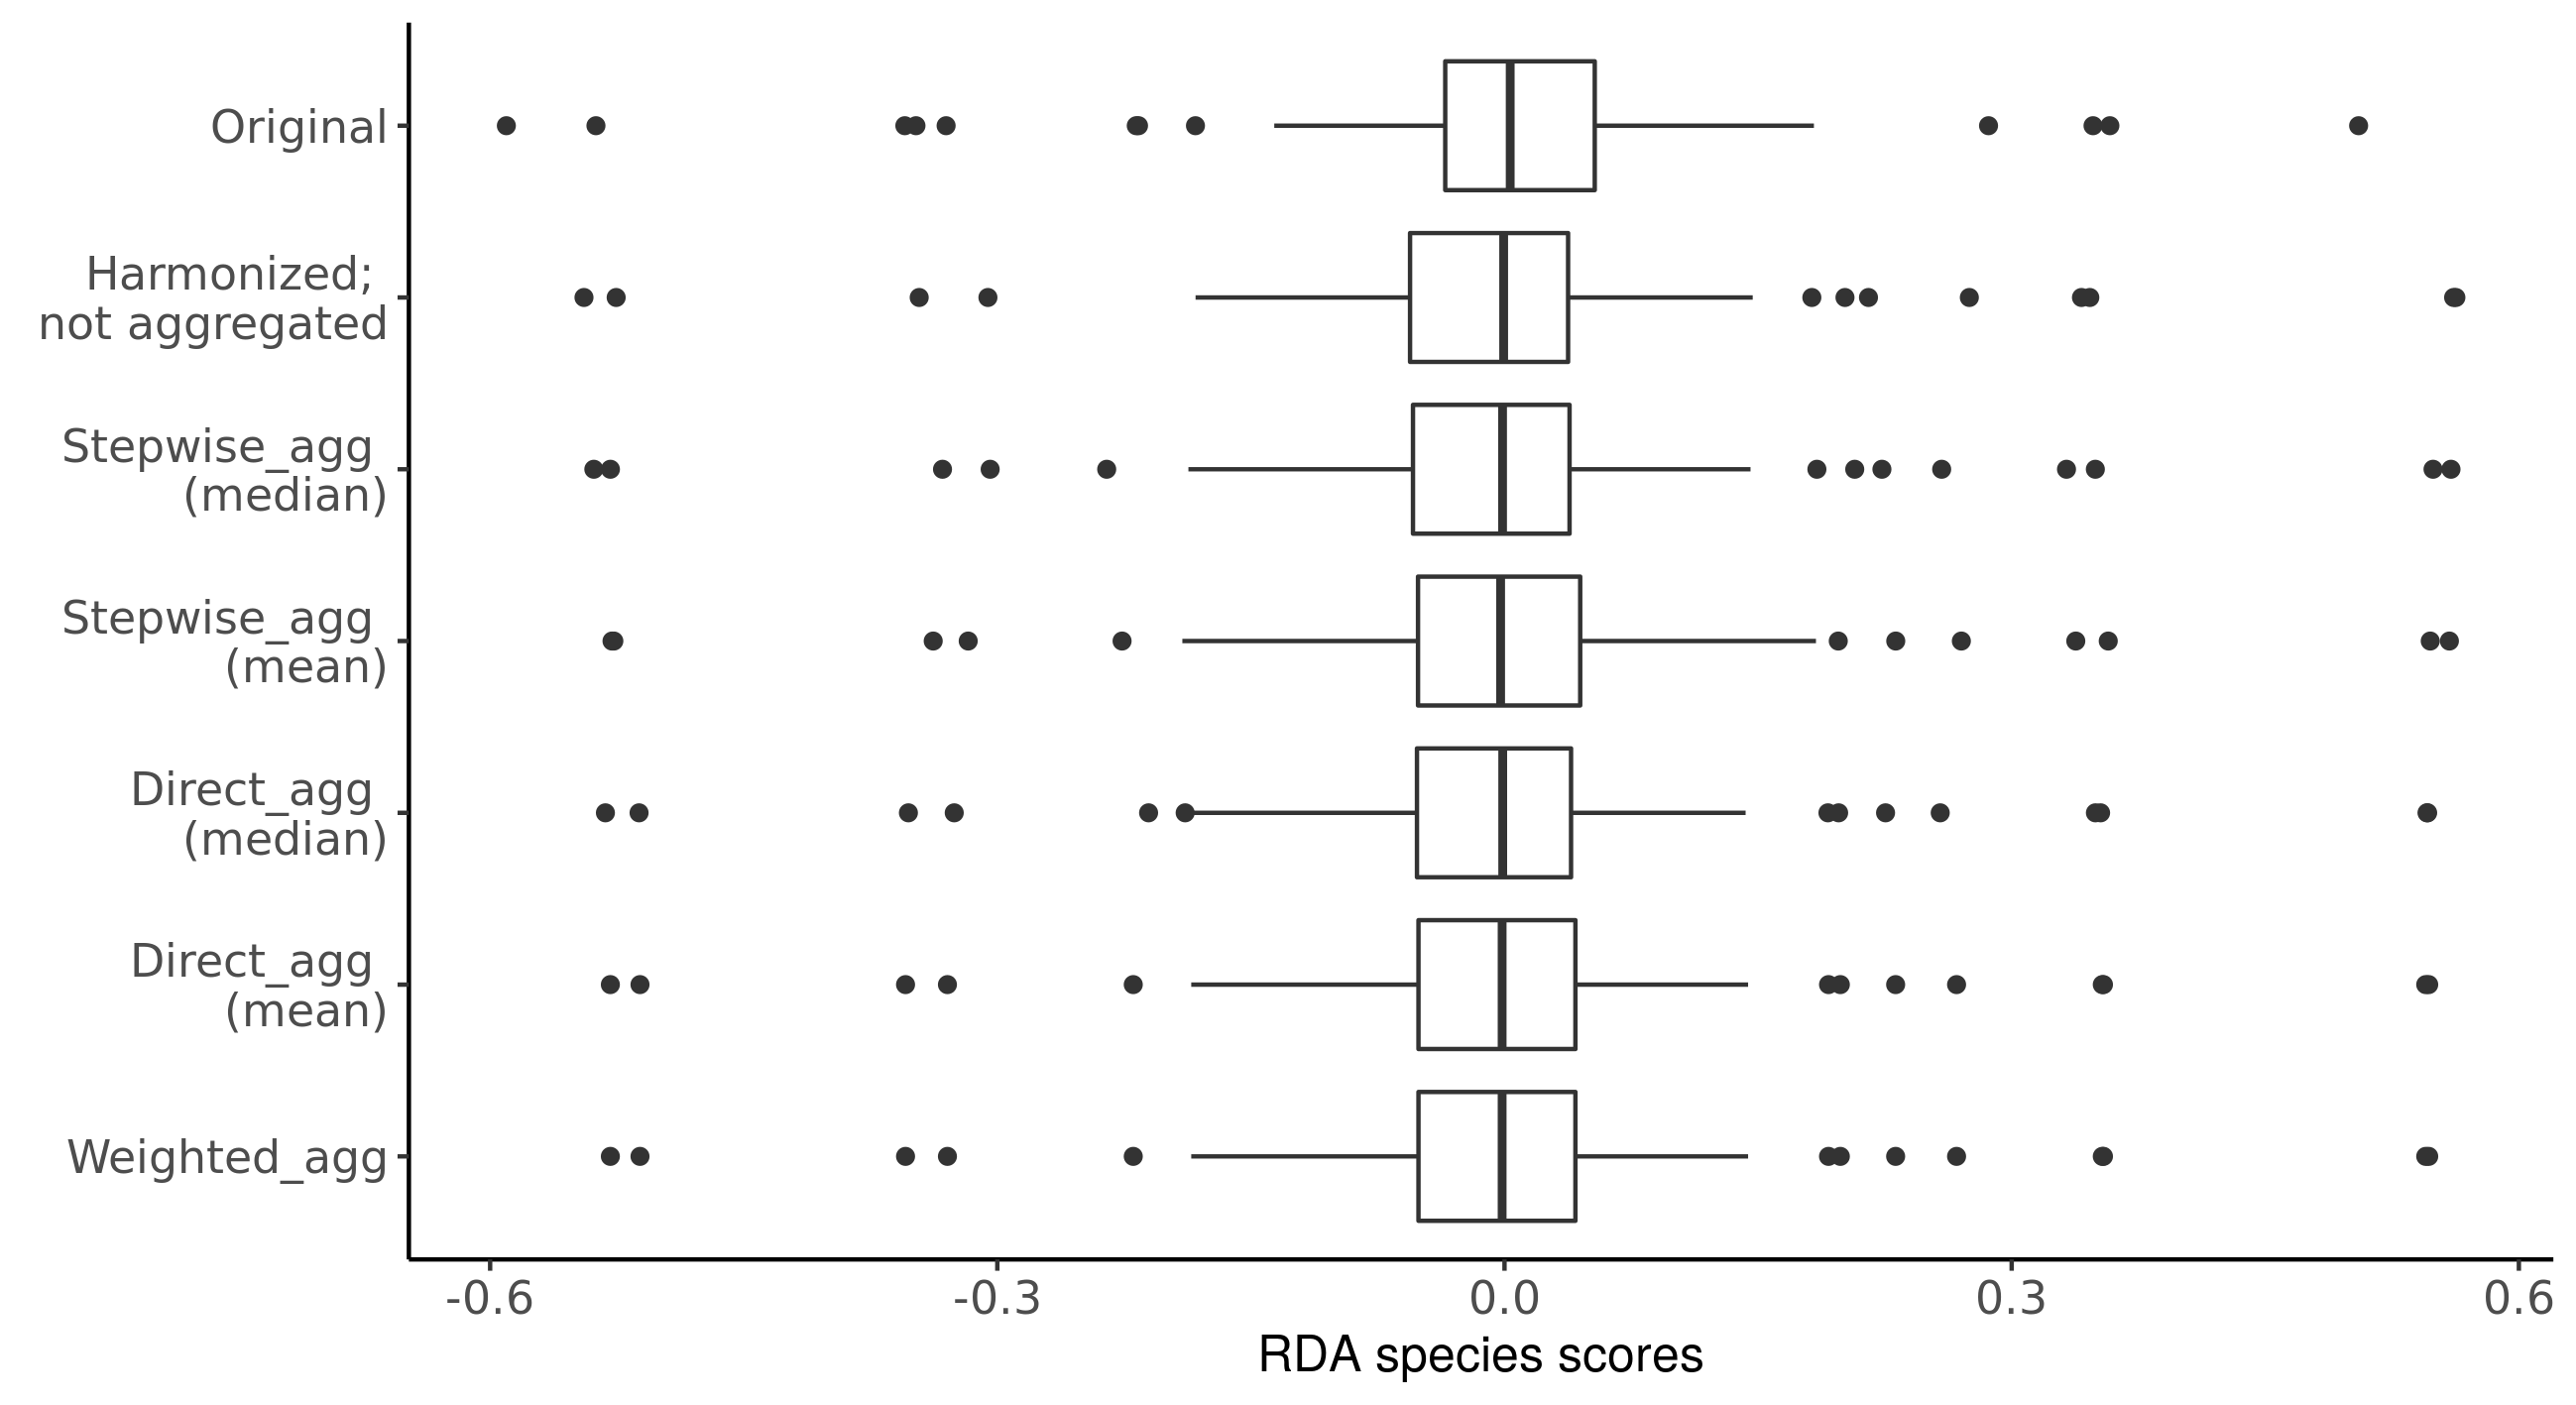
\includegraphics[width=16.5cm, height=10cm]{Species_scores_rda.png}
    \caption{Species scores obtained by RDA from the original analysis \cite{szocs_effects_2014}, using harmonized grouping features, and using harmonized grouping features with traits aggregated to family-level. The dots represent the individual species scores for each analysed trait. The violin plot shows the density estimate of the species scores. Gray vertical lines indicate the median of the obtained species scores.}
\end{figure}

\begin{sidewaysfigure}
  \label{fig:boxplots_scores_on_constrained_axis}
  \centering
  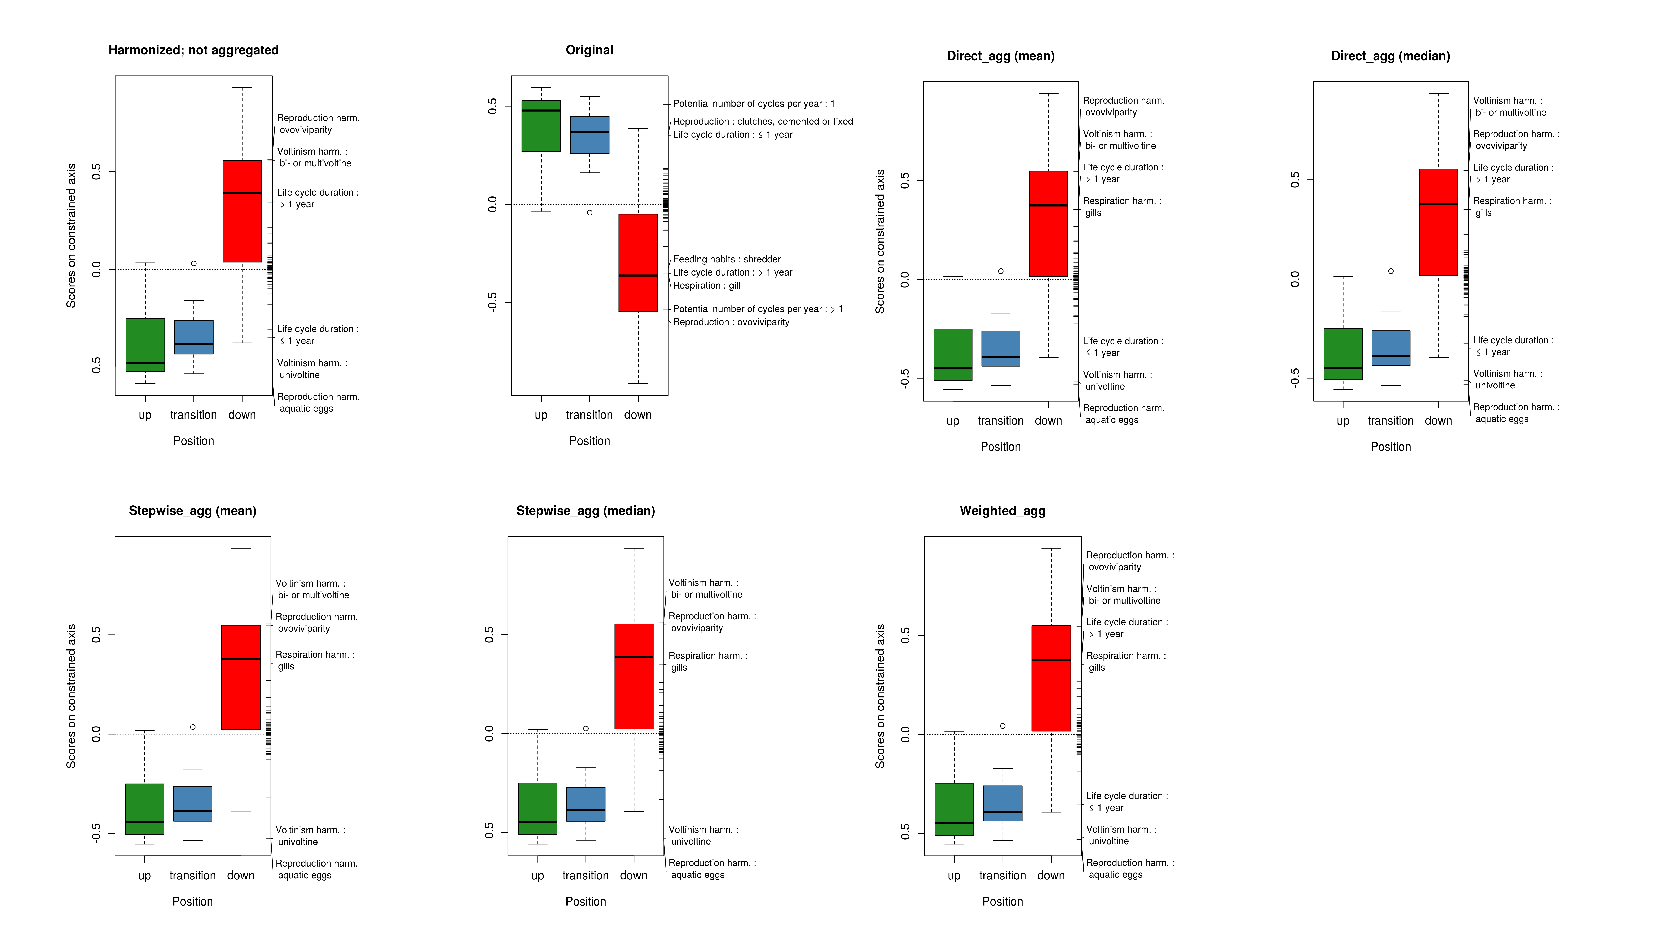
\includegraphics[width= 22cm, height=12cm]{Scores_on_constrained_axis_combined.pdf}
  \caption{RDA of traits constrained by electric conductivity for the tested methods and the original study. Shown are boxplots of the site scores along the conductivity axis. The rug on the right side of each plot indicates species scores of the traits on the conductivity axis. Only traits with a mahalanobis distance greater than the $97.5 \%$ quantile of the Chi-square distribution (5.02) were labelled.}
\end{sidewaysfigure}

\newpage

%%%%%%%%%%%%%%%%%%%%%%%%%%%%%%%%%%%%%%%%%%%%%%%%%%%%%%%%%%%%%%%%%%%%%%%%%%%%%%%%%%%%%%%%%%%%%%%%%%%%

\subsection*{Discrepancies of invertebrate trait definitions}

Definitions of grouping features and traits varied in their level of detail in the original trait databases. The freshwaterecology.info database, the Tachet database and the North American database (Twardochleb et al.) provided more detailed descriptions of their trait information compared to the North American (Vieira et al.) and New Zealand database. An exception is the Australian trait database which is a collection of seven specific trait datasets \cite{kefford_integrated_2020}. Thus, grouping features occur multiple times with varying differentiation into traits. Depending on the dataset trait information is described with more or less detail.

The definition of grouping features varied across databases mainly concerning their differentiation into traits but also in their scope. We provide a summary of discrepancies in trait definitions in the appendix (Table S\ref{stab:trait_definitions}). Both, differences in differentiation and scope can lead to discrepancies in trait definitions. For example, for the grouping feature feeding mode discrepancies arise because traits are assigned in different ways. The Tachet database defines predators as carvers, engulfers and swallowers. By contrast, in the North American (Twardochleb et al.) database predators are defined as engulfers and carnivorous piercers. In turn, in the Tachet database, piercers are defined as a separate trait encompassing herbivorous and carnivorous piercers. Furthermore, the scope in the freshwaterecology.info database for feeding mode is primarily on the food source of a species (except for filterers), while the other databases focus on the strategies of food acquisition. Therefore, the freshwaterecology.info database defines e.g. predator as "eating from prey", while the other databases use the mouthpart morphology as basis of their definition. The Tachet database captures the food source in an additional grouping feature. Varying levels of differentiation are also present in all other investigated grouping features between the trait databases (Table \ref{tab:trait_databases_coding_differentiation} and Table S\ref{stab:trait_definitions}). Locomotion definitions differ also in scope between databases. Freshwaterecology.info and New Zealand databases describe locomotion as the way of movement of an organism, Tachet as substrate relation and locomotion, the North American (Vieira et al.) as how organisms deal with flow, Australia as attachment, and the North American (Twardochleb et al.) database includes not only the way of movement, but also the location of movement. Similarly, regarding the reproduction traits, databases differ in their scope. Reproduction is captured in one grouping feature and defined as location of oviposit clutches and mode of reproduction in the freshwaterecology.info and Tachet databases. North America (Vieira et al.) provides information on the oviposition location but not on reproductive behavior. The Australian database report traits for reproductive behavior but also on oviposition site. The New Zealand database distinguishes three grouping features related to reproduction: reproductive technique, oviposition site (e.g. water surface, terrestrial), and egg/egg mass (e.g. free, cemented).

Various codings of traits are used throughout the databases (e.g. binary, fuzzy, continuous). The freshwaterecology.info and Australian use different codings in their databases. Tachet and the New Zealand database exclusively use fuzzy coding. Both North American trait databases contain categorical grouping features that can be converted into traits using a binary coding (Table \ref{tab:trait_databases_coding_differentiation}). Binary coding represents a simple approach in which a taxon either expresses a trait or not. Fuzzy coding characterizes the affinity of an organism to exert a certain trait. It is used to account for plasticity in traits, e.g. taking into account that traits can change over the development time of an organism. Usually, fuzzy coded affinities are converted into proportional values. Continuous coding is used for traits like body size.
% Last sentences are a bit redundant

% None of the seven grouping features compared here has the same differentiation of traits across all databases (Table \ref{tab:trait_databases})
\begin{landscape}
    \begin{longtable}{m{2.5cm}|m{1.8cm}|m{2.3cm}|m{1.8cm}|m{3cm}|m{2cm}|m{2cm}|m{1.8cm}}
    \caption{Number of traits per grouping feature and type of coding of the traits for the respective grouping feature per database.}
    \endfirsthead
    \toprule[.1em]
    \label{tab:trait_databases_coding_differentiation}
    Database & Feeding Mode & Voltinism & Locomotion & Respiration & Reproduction & Size & Body Form \\ 
    \toprule[.1em]
    \multirow{2}{*}[-5mm]{ \specialcell{Freshwater- \\ ecology.info}} & 
    10 & 
    6 &
    6 & 
    7 & 
    9 & 
    - & 
    - 
    \\
    \cline{2-8} & 
    \specialcell{10 point \\ assignment \\ system} &
    \specialcell{single category \\ assignment \\ system} &
    \specialcell{10 point \\ assignment \\ system} &
    \multicolumn{2}{c |}{\specialcell{binary}} &
    - & 
    - \\
    \hline
    \hline
    \multirow{2}{*}{Tachet} & 
    7 & 
    3 &
    8 & 
    5 & 
    8 & 
    7 & 
    - 
    \\
    \cline{2-8} &
    \multicolumn{2}{c |}{fuzzy $[0-3]$} &
    fuzzy $[0-5]$ & 
    \multicolumn{3}{c |}{fuzzy $[0-3]$} & 
    -
    \\
    \hline
    \hline
    \multirow{2}{*}{\specialcell{North America \\ (Twardochleb)}} & 
    6 & 
    3 &
    10 & 
    3 & 
    10 & 
    3 & 
    - 
    \\
    \cline{2-8} &
    \multicolumn{6}{c |}{binary} &
    -
    \\
    \hline
    \hline
    \multirow{2}{*}{\specialcell{North America \\ (Vieira)}} & 
    8 & 
    3 &
    9 & 
    8 & 
    10 & 
    3 & 
    5 
    \\
    \cline{2-8} &
    \multicolumn{7}{c }{binary}
    \\
    \hline
    \hline
    \multirow{2}{*}[-4mm]{Australia} & 
    16 \textsuperscript{\textit{a}} & 
    7 &
    9 & 
    10 &
    13 \textsuperscript{\textit{b}} & 
    9 & 
    4
    \\
    \cline{2-8} & 
    \multicolumn{2}{c |}{\specialcell{binary; proportional $[0 - 1]$; \\ fuzzy $[0 - 3]$}} & 
    binary; fuzzy $[0 - 3]$ & 
    \specialcell{binary; proportional \\ scale $[0 - 1]$; \\ fuzzy $[0 - 3]$} & 
    categorical & 
    \specialcell{binary; \\ continuous; \\ fuzzy $[0 - 3]$} & 
    fuzzy codes $[0-3]$
    \\
    \hline
    \hline
    \multirow{2}{*}{New Zealand} & 
    6 & 
    3 & 
    4 & 
    4 & 
    4 & 
    5 & 
    4
    \\
    \cline{2-8} & 
    \multicolumn{7}{c }{fuzzy $[0-3]$}
    \\
    \bottomrule
    \end{longtable}
    \begin{minipage}{\linewidth}\small
        \textit{a} Some of the traits were similar (e.g. trait \textit{Shredder}, \textit{Shredder, Detrivore}, and \textit{Collector, Shredder}).
        \newline
        \textit{b} Many traits were rather comments than traits in the original database and were not considered.
    \end{minipage}
\end{landscape}

%%%%%%%%%%%%%%%%%%%%%%%%%%%%%%%%%%%%%%%%%%%%%%%%%%%%%%%%%%%%%%%%%%%%%%%%%%%%%%%%%%%%%%%%%%%%%%%%%%%%

\section*{Discussion}

\subsection*{Differences in trait affinities obtained by trait aggregation methods compared to traits assigned at family-level}


% Summarize briefly results and synthesize (with Simulation)  
Our results show that aggregation of traits by the median compared to aggregating by the mean is often closer to the assigned traits at family level, i.e. it yields less differing cases. 
% This part needs to be improved:
% However, aggregation methods using the median tend to produce greater differences between aggregated and assigned traits.
The different weighting methods, i.e. aggregating stepwise, direct or weighted, did not seem to have a strong impact, because the distribution of absolute trait affinity differences to assigned traits obtained by the \textit{direct\_agg\textsubscript{mean}}, \textit{stepwise\_agg\textsubscript{mean}} and \textit{weighted\_agg} were relatively similar in both tested datasets.  %as well as for direct\agg (median) and stepwise\_agg (median)
Instead, using the mean or the median changed the distribution of differences in trait affinities between aggregated and assigned traits.
% Wording!
A reason that using different weightings for the taxa when aggregating doesn't seem to have a big influence is on the one hand, that the used taxa had only a low number of genera in the used trait datasets or don't have species entries at all. From the taxa that were compared from the North American trait dataset to the assigned traits at family-level, 13.8 \%, 61.7 \% were resolved on genus-level. 52.1 \% had 5 or less genera and 12.8 \% contained just one genus (Figure S\ref{fig:tax_hierarchy_NOA}). In the Australian dataset 21.4 \% of the compared taxa had trait information resolved on family-level, 39.5 \% resolved on genus level, and 39.1 \% resolved on species-level. 67.73 \% of the taxa contain 5 or less genera and 39.6 \% just contained one genus (Figure S\ref{fig:tax_hierarchy_AUS}). The simulation results indicated that the choice of the aggregation method for small numbers of genera per family (5) can be important when one genus has a much larger number of species compared to other genera within a particular family. 
% How often in the trait datasets?
However, inspecting the simulated datasets revealed that often aggregated traits only differ slightly obtained from the different aggregation methods .

% Differences between datasets 
Observed differences between aggregated and assigned traits were higher for the North American trait dataset. This can be explained by the binary coding of the traits in the North American dataset. As a results, traits have been assigned affinities of either 1 or 0. Thus naturally, even after normalization, traits of a particular grouping feature have a high difference of trait affinities to each other compared to when they were coded using fuzzy codes.

% Of course all the comparisons have no "generellen Gültigkeisanspruch" - what's the true aggregated trait affinity characterising a particular family? Expert assignments maybe also biased based on experience with a particular group of taxa within a family.  
Evaluation of the differences between aggregated and assigned traits is difficult because it remains unclear what the true value of a particular trait for a particular organism on family-level is. It is indeed questionable whether the aggregation of trait information on species or genus-level to a point estimate on family-level can be an adequate description of a particular trait at all, especially for traits with a high variability. In fact, traits can vary strongly on more precise taxonomic levels than the family-level. For example, Monaghan and Soares found a high dispersion of trait affinities at genus-level within families in the Tachet database for traits of the grouping features body size, flow preference, and reproduction \cite{monaghan_improving_2013}. Furthermore, studies focusing on the lability of traits, i.e. how much traits are unconstrained by phylogeny, found that traits of ecological preferences (e.g. thermal preference), body size, resistance forms, and to a lesser extent feeding mode are labile, and thus possibly highly variable \cite{poff_functional_2006,wilkes_traitbased_2020}. Thus, it is likely that assigned traits and aggregated traits at family-level will especially differ in affinities for the aforementioned traits. Our analysis could confirm this partially. The highest possible difference of 1 between aggregated trait affinities and assigned trait affinities (in total in 6.9 \% of all cases) for the Australian dataset occurred most often for body size large and medium (42.5 \% and 39.2 \% of all cases with a difference of 1, respectively) across all comparisons. Both traits had also the highest mean and standard deviation in the absolute difference of trait affinities across all tested comparisons (mean size medium 0.5, sd 0.29; mean size large 0.59, sd 0.32). For the taxa compared from the North American dataset, the highest possible difference in trait affinities occurred most often for the trait body size medium (15.8 \% of all cases with a maximum difference), followed by the traits respiration via plastron and spiracle and respiration via tegument (both 13 \% of all cases with a maximum difference). Respiration via plastron and spiracle showed the highest mean and standard deviation in the absolute difference of trait affinities across all comparisons (mean 0.71, sd 0.33), followed by respiration via tegument (mean 0.5, sd 0.34) and body size medium (mean 0.49, sd 0.3). 

% Outlook: combine trait information for priors like in species distribution models/population growth models,
% see Kindvater et al and Brown & Roff 
% ? Constructing priors from fuzzy coded traits



% Further ideas: 
%   - Differences across grouping features
%   - Still some similarities between compared datasets -> Where does the classification come from?
%     Few sources used in NOA also used in AUS:
%     AUS: Merrit & Cummins 1978/1984 for feeding mode for a few genera and families 
%     NOA: Merritt, Richard W., Cummins, Berg 2008 -> but not clear if for feeding mode as well; according to trait   %     description "Cummins, K. W. Trophic Relations of Aquatic Insects" was used
%   - Could not include all data due to data gaps -> much needed to be filled -> would maybe change the picture?

\subsection*{Re-analysis of Szöcs et al. using harmonized and aggregated grouping features}

% Were the traits promoted by the harmonized dataset on the most extreme points on the conductivity axis?
% Large scale studies?

% What does this imply for future studies -> return to the introduction


\begin{itemize}
  \item \textbf{aggregated vs assigned traits}
  \begin{itemize}
    \item In general, differences produced by the aggregation methods seem to arise by using mean or median, not so much driven by the different weighting approaches (direct vs. stepwise vs. weighted)
    \item Approaches that used the median resulted in fewer differences to the assigned traits, albeit if differences occurred to the assigned traits, they were greater. 
    \item Simulation shows that approaches using the median generally produce a larger range of values $\rightarrow$ Especially with higher trait variability for situations where one genus has a lot more species than the other genera within the family 
    \item Differences greater for the NOA dataset because of the binary coding $\rightarrow$ differences are greater between traits
    \item Taxonomic hierarchy in the investigated datasets? \\
     $\rightarrow$ In every investigated dataset families have only 1 to few genera. 76 (North America) to 93 \% (New Zealand) of the families have 5 or less genera (see SI). 
    \item There is no "true" value to compare to, i.e. assigned traits at genus or family level can be biased as well (i.e. the person who assigned the trait was thinking about particular species within a genus not all). Comparison of species-level traits in fwe and traits on genus-level in tachet would be interesting in this context? 
    \item  Suggestions from Co-Authors: \\
     $\rightarrow$ should include where the classifications come from \\
     $\rightarrow$ what do we really know because someone has watched the animals and published their behaviour; what is extrapolated knowledge? \\
     $\rightarrow$ are the differences between continents because of evolution or only because scientists have done more research in one of the continents?
  \end{itemize}
  \item \textbf{Influence of aggregation methods on trait-environment relationships}
  \begin{itemize}
    \item We re-analysed only a small-scale study, what would be different when applying a large-scale study?
  \end{itemize}
\end{itemize}

% Discussion point BK: It is intersting that Australia has fewer species and genus than NOA and EU (not suprisngly since the datasets in Oz were mostly delveoped at family level) but more families than these other regions. I wonder if this indicates that Family richness is really higher in Australia. Perhaps it might be as Australia has a wider range of evolutionary histories. This would be worth considering in the discussion

% 2) Influence of aggregation methods on trait-environment relationships: 
% Harmonization: Minor influence on RDA species scores
% RDA species scores 
%   -> Normalized eigenvectors
%   -> dependent on nr. of variables? Nr. of response variables not really influential 
% We used only a small-scale study -> What's different to large-scale studies?
% Further aggr. after harmonization: no difference to the harmonized dataset
% ?Logical because trait aggr. methods themselves showed only minor differences
% Complex Stat. techniques developed -> cannot use full potential

\newpage

%%%%%%%%%%%%%%%%%%%%%%%%%%%%%%%%%%%% Bibliography %%%%%%%%%%%%%%%%%%%%%%%%%%%%%%%%%%%%%%%%%%%%%%%%%%%%%
\printbibliography

\newpage

%%%%%%%%%%%%%%%%%%%%%%%%%%%%%%%%%%%% Supporting information %%%%%%%%%%%%%%%%%%%%%%%%%%%%%%%%%%%%%%%%%%%
\setcounter{table}{0}
\setcounter{figure}{0}

\subfile{Results/SI}

\end{document}